\section{Testování frameworků}

V rámci této kapitoly se zaměříme na testování tří vybraných frameworků. V první části navrhneme funkční a nefunkční požadavky demonstračních aplikací. 
Následně vytvoříme demonstrační aplikaci, která bude obsahovat stejné funkcionality ve všech třech vybraných frameworcích. 
V poslední části srovnáme implementaci aplikací, identifikujeme přednosti a nedostatky použitých frameworků. 

\subsection{Návrh aplikace}

Začneme návrhem aplikace, kterou později implementujeme v rámci vybraných frameworků. 
Webová aplikace se bude skládat z několika stránek, které zobrazí navrhnuté funkcionality. 
Ty následně poslouží při porovnání přístupu a implementace jednolivých nástrojů.

\subsubsection{Funkční požadavky}

\begin{citemize}
	\item Správa stavů, předávání vlastností -- Counter komponenta:
	
	\begin{cenumerate}
		\item Uživateli bude zobrazen aktuální stav čítače.
		\item Uživateli bude umožněno zvýšit a snížit hodnotu čítače o 1.
		\item Uživatel bude mít možnost resetovat hodnotu čítače na 0.
	\end{cenumerate}

	\item Interakce v uživatelském prostředí -- Dropdown komponenta:
	
	\begin{cenumerate}
		\item Komponenta bude zobrazovat rozbalovací menu.
		\item Po kliknutí na menu se zobrazí seznam položek.
		\item Uživatel bude mít možnost vybrat jednu z položek, nebo zavřít menu.
		\item Aktuálně vybraná položka bude zobrazena v obsahu rozbalovacího menu.
	\end{cenumerate}

	\item Reaktivita, asynchronní operace -- Translator komponenta:
	
	\begin{cenumerate}
		\item Uživatel bude mít možnost zadat text, který chce přeložit.
		\item Uživatel bude mít možnost vybrat jazyk, do kterého chce text přeložit.
		\item Přeložený text získáme díky veřejnému API.
		\item Uživateli bude zobrazen přeložený text.
		\item V případě chyby při překladu bude uživateli zobrazena chybová hláška.
	\end{cenumerate}

	\item Tvorba formulářů, validace -- InvestForm komponenta:
	
	\begin{cenumerate}
		\item Komponenta bude zobrazovat formulář pro výpočet výnosu investice.
		\item Uživatel bude mít možnost zadat vstupní hodnoty formuláře.
		\item Formulář bude obsahovat validaci vstupních hodnot a nedovolí uživateli potvrdit formulář s jakoukoli nevalidní hodnotou formuláře.
		\item Po potvrzení formuláře bude provedena kalkulace výsledků a ty budou zobrazeny uživateli.
	\end{cenumerate}

	\item Modularita, použití knihoven -- CountryGuesser komponenta:
	
	\begin{cenumerate}
		\item Data o zemích získáme pomocí veřejného API.
		\item V rámci hry bude náhodně vybrána země, kterou bude uživatel hádat.
		\item Uživateli se v rámci hry budou postupně zobrazovat informace (nápovědy) o hádané zemi.
		\item Uživatel bude mít možnost zadat či vybrat pouze existující název země, který chce tipovat.
		\item Uživatel následně uvidí již zadané země a vzdálenost jím dané země od hádané země.
		\item Uživateli bude při výhře a prohře zobrazeno modální okno s informacemi o výsledku hry.
		\item V případě chyby při získávání dat o zemích bude uživateli zobrazena chybová hláška.
	\end{cenumerate}

	\item Routování a layout aplikace:
	
	\begin{cenumerate}
		\item Uživatel bude umožněna navigace mezi jednotlivými stránkami aplikace.
		\item Uživatel bude mít možnost zapnout a vypnout tmavý režim aplikace.
	\end{cenumerate}
\end{citemize}

\subsubsection{Nefunkční požadavky}

\begin{citemize}
	\item Webová aplikace bude uživatelsky přívětivá.
	\item Webová aplikace bude responzivní a bude se správně zobrazovat na různých zařízeních.
	\item Implementace bude dodržovat principy čistého kódu, také principy KISS, DRY a SOLID.
	\item Aplikace bude získávat data z veřejných API.
	\item Při implementaci budeme dbát na použití moderních technologií a nástrojů.
	\item Budou využity open source knihovny, nástroje a ikony. 
\end{citemize}

\subsection{Implementace webových aplikací}

V této kapitole popíšeme implementaci jednotlivých částí aplikace v rámci vybraných frameworků. Použijeme následující nástroje v níže uvedených verzích:

\begin{citemize}
	\item Angular -- verze 17.x.x
	\item React -- verze 18.x.x
	\item Svelte -- verze 4.x.x
\end{citemize}

Pro grafickou stránku aplikací využijeme CSS framework Tailwind CSS \cite{tailwindcssframework} a ikony od tvůrců Tailwind CSS -- Heroicons \cite{heroiconslib}. 
Obě knihovny jsou open source a zdarma k použití pod licencí MIT License. 
K vytvoření nového projektu v jednotlivých frameworcích budeme potřebovat NodeJS a správce balíčků npm (případně jiného správce balíčků).

\begin{table}[htb]
	\centering
	\caption{Instalace projektů v jednotlivých frameworcích.}
	\medskip
	\radkovani[1.2]
		\begin{tabular}{|l|l|}
		\hline
		\textbf{Framework} & \textbf{Příkazy pro instalaci} \\ \hline
		Angular   & \begin{tabular}[c]{@{}l@{}}npm init @angular@latest nazev-projektu\\ cd nazev-projektu\\ npm install -D tailwindcss postcss autoprefixer\\ npx tailwindcss init -p\\ manuální konfigurace Tailwind CSS\footnotemark[1]\\ npm run start\end{tabular} \\ \hline
		React     & \begin{tabular}[c]{@{}l@{}}npm create vite@latest\\ cd nazev-projektu\\ npm install -D tailwindcss postcss autoprefixer\\ npx tailwindcss init -p\\ manuální konfigurace Tailwind CSS\footnotemark[2]\\ npm run dev\end{tabular}       							\\ \hline
		Svelte    & \begin{tabular}[c]{@{}l@{}}npm create vite@latest\\ cd nazev-projektu\\ npx svelte-add@latest tailwindcss\footnotemark[3]\\ npm install\\ npm run dev\end{tabular}                                                                                 	\\ \hline
		\end{tabular}
	\label{tab:test}
\end{table}

\footnotetext[1]{Konfigurace Tailwind CSS v Angular projektu dle oficiální dokumentace.\cite{twconfigangular}}
\footnotetext[2]{Konfigurace Tailwind CSS v React projektu dle oficiální dokumentace.\cite{twconfigreact}}
\footnotetext[3]{Automatická instalace Tailwind CSS ve Svelte projektu pomocí svelte-add balíčku.\cite{twconfigsvelte}}

\subsubsection{Angular}

\begin{flushleft}
  \textbf{Správa stavů, předávání vlastností}
\end{flushleft}

Pro implementaci jednoduchého counteru nejprve vytvoříme counter komponentu. Můžeme začít se strukturou HTML značek pro hlavní komponentu.

\begin{prog}
// Soubor counter.component.html

<div class="bg-gray-200 p-6 rounded-md shadow-md">
  <p class="text-xl font-semibold mb-4">Current count: \{\{ count \}\}</p>

  <div class="flex gap-4">
    <counter-button
      [className]="'bg-blue-500 text-white hover:bg-blue-600'"
      (buttonClicked)="increment()"
    >
      Increment
    </counter-button>

    <!-- další tlačítka... -->
  </div>
</div>
\end{prog}

Jelikož potřebujeme opakovaně použít logiku jednotlivých tlačítek, vytvoříme komponentu counter-button. 
Ta může přijímat například CSS styly nebo přes output (\emph{EventEmitter}) posílat informaci o~kliknutí na tlačítko směrem nahoru ve stromě komponent.

\begin{prog}
// Soubor counter-button.component.ts

import \{CommonModule\} from '@angular/common';
import \{Component, EventEmitter, Input, Output\} from '@angular/core';

// Nastavení komponenty.
@Component(\{
  selector: 'counter-button',
  standalone: true,
  templateUrl: './counter-button.component.html',
  imports: [CommonModule],
\})
export class CounterButtonComponent \{
  // Vstupní vlastnost komponenty.
  @Input() public className = '';

  // Výstupní vlastnost komponenty.
  @Output() public buttonClicked = new EventEmitter<void>();
\}
\end{prog}

Funkci \emph{emit()} \emph{EventEmitteru} zavoláme na tlačítku v~counter-buttonu právě tehdy, když uživatel klikne na tlačítko -- použijeme listener ve formě \emph{(click)}. 
K~propsání textu či jiných elementů nebo komponent mezi párovými tagy <counter-button> pak poslouží párový či nepárový element <ng-content />.

\begin{prog}
// Soubor counter-button.component.html

<button
  class="px-4 py-2 rounded-md focus:outline-none"
  [ngClass]="className"
  (click)="buttonClicked.emit()"
>
  <!-- ng-content slouží k vykreslení obsahu, který vložíme
    mezi párové tagy (selectory) dané komponenty. -->
  <ng-content></ng-content>
</button>
\end{prog}

Následně v~counter komponentě importujeme třídu CounterButtonComponent a~do všech elementů counter-button předáme jejich vstupy a~výstupy. 
Námi definovanovanému outputu \emph{buttonClicked} předáme v~šabloně metodu, která se vykoná po emitu (kliknutí na tlačítko ve vnořené komponentě) a~metodu zavoláme pomocí kulatých závorek. 
V~rámci counter komponenty pak definujeme stav jako vlastnost \emph{count} na třídě. Vlastnost pak můžeme modifikovat skrze metody třídy, které voláme v~outputu \emph{buttonClicked}.

\begin{prog}
// Soubor counter.component.ts

import \{CommonModule\} from '@angular/common';
import \{Component\} from '@angular/core';
import \{CounterButtonComponent\} from './button/counter-button.component';

@Component(\{
  selector: 'counter',
  standalone: true,
  templateUrl: './counter.component.html',
  imports: [CommonModule, CounterButtonComponent],
\})
export class CounterComponent \{
  protected count = 0;

  protected increment(): void \{
    this.count++;
  \}

  protected decrement(): void \{
    this.count--;
  \}

  protected reset(): void \{
    this.count = 0;
  \}
\}
\end{prog}

\begin{flushleft}
  \textbf{Interakce v uživatelském prostředí}
\end{flushleft}

Při vytváření jakékoli UI komponenty můžeme začít šablonou, nebo definovat funkční stránku. My začneme s~tvorbou šablony. V~případě vlastního dropdown samotným tlačítkem a~seznamem možností. 
Otevření možností zajístíme tak, že na tlačítko přidáme click listener. Funkčnost pak zajistíme díky modifikaci stavu \emph{isOpen}, který se provede při volání metody \emph{toggleDropdown}. 
V~rámci této metody je třeba zavolat i~\emph{event.stopPropagation()}. Předejdeme tak potenciální chybě ve formě tzv. event bubblingu -- spuštění událostí na prvcích odlišných od cílového.

\begin{prog}
// Část souboru dropdown.component.html

<div class="rounded-md shadow-sm">
  <!-- Pro poslouchání na události v DOMu můžeme 
    použít syntaxi: (NÁZEV_UDÁLOSTI)="OBSLUŽNÁ_METODA". -->
  <button
    type="button"
    class="" <!-- Statické styly... -->
    [ngClass]="buttonStyles + ' ' + sizeStyles"
    (click)="toggleDropdown(\$event)"
  >
    \{\{ selectedOption ? selectedOption.label : placeholder \}\}
    <!-- Pro podmíněné vykreslovaní můžeme využít bloky @if, @else if, @else. -->
    @if (isOpen) \{
      <arrow-up-icon />
    \} @else \{
      <arrow-down-icon />
    \}
  </button>
</div>
\end{prog}

Podmíněně zobrazíme seznam možností, které získáme v~jednom z~inputů. K~vykreslení všech možností použijeme blok \emph{@for}. 
Pro vybraní konkrétní možnosti využijeme \emph{(click)} a~do obslužné metody předáme aktuální prvek v~poli -- option. 
Metoda \emph{handleOptionClick} pak zajistí uložení aktuálně vybrané možnosti, zavření dropdownu a~vyemitování vybrané možnosti do rodičovské komponenty.

\begin{prog}
// Část souboru dropdown.component.html

@if (isOpen) {
  <div
    class="" <!-- Statické styly... -->
    [ngClass]="divStyles"
  >
    <div class="py-1" role="menu"> <!-- WAI-ARIA atributy... -->
      <!-- Pro vykreslení listu (pole hodnot) můžeme využít blok @for. -->
      @for (option of options; track option.value) {
        <button
          class="block w-full text-left px-4 py-2 text-sm hover:text-gray-900"
          [ngClass]="optionStyles"
          role="menuitem"
          (click)="handleOptionClick(option)"
        >
          {{ option.label }}
        </button>
      }
    </div>
  </div>
}
\end{prog}

V~případě, že máme dropdown otevřen a~chceme jej po kliknutí mimo tentýž dropdown bezpečně zavřít, nehledě na počet vykreslených dropdown komponent na stránce, budeme postupovat následovně. 
Pro každou komponentu vytvoříme unikátní vlastnost ve formě ID. To pak dynamicky umístíme na kořenový element dropdownu.

\begin{prog}
// Část souboru dropdown.component.ts

protected dropdownId = `id-\${crypto.randomUUID()}`;

// Část souboru dropdown.component.html

<div class="relative inline-block text-left" [id]="dropdownId">
\end{prog}

V~komponentě pak budeme naslouchat na události v~DOM pomocí dekorátoru \emph{@HostListener}. 
Dekorátor přijímá DOM událost, na který má poslouchat -- \emph{document:pointerdown}, případně další argumenty nebo také formu vypublikované události. 
Pod dekorátorem pak definujeme obslužnou metodu, která se volá při emitu specifikované události. V~rámci metody pak zajistíme uzavření aktuálně otevřeného dropdownu.

\begin{prog}
// Část souboru dropdown.component.ts

@HostListener('document:pointerdown', ['\$event.target'])
onClickOutsideDropdown(target: HTMLElement): void \{
  if (this.isOpen && !target.closest(`#\$\{this.dropdownId\}`)) \{
    this.isOpen = false;
  \}
\}
\end{prog}

Dropdown pak může mít různé inputy, které povedou k~lepší znovupoužitelnosti. Hodnotu inputu (konkrétně např.~\emph{defaultValue}) v~komponentě získáme v~metodě životního cyklu \emph{OnInit}. 
Styly ve formě JS hodnot do šablony přidáme pomocí \emph{ngClass}. Když těchto hodnot potřebujeme na elementu více, zřetězíme předávané hodnoty pomocí JavaScriptu. 
Další možnost spočívá ve sloučení požadovaných stylů na úrovni třídy.

\begin{flushleft}
  \textbf{Reaktivita, asynchronní operace}
\end{flushleft}

Pro ukázku reaktivity a~asynchronních operací můžeme vytvořit komponentu, která bude překládat zadaný text do vybraného jazyka. 
Začneme tedy vytvořením rodičovské komponenty, která při změně vlastností (zadaného textu uživatelem a~výstupního jazyka) zavolá API, které vrátí přeložený text. 
V~rámci této komponenty vytvoříme vnořené komponenty, které budou sloužit k~zadání vstupního textu, výběru jazyka a~zobrazení výsledku. 

LanguageDropdownComponent umožní uživateli vybrat jazyk, do kterého chce přeložit text. 
Přes \emph{EventEmitter} aktualizujeme výstupní jazyk v~rodičovské komponentě. V~rámci obslužné metody \emph{handleLanguageChange} pak také modifikujeme hodnotu vlastnosti \emph{inputValuesChanges\$}.
Tato vlastnost je \emph{Subject}, speciální typ observable, z~knihovny RxJS. Později dovolí na základě změny hodnoty poslat dotaz na server ve správný moment. 
Podobným způsobem poté můžeme registrovat událost změny vstupního textu -- naslouchat na změnu vstupního textu.
% TODO: Přidat schéma

\begin{prog}
// Část souboru translator.component.ts

protected handleLanguageChange(outputLanguage: Option): void \{
  this.outputLanguage = outputLanguage.value;
  // Synchronní aktualizace hodnoty observable (v tomto případě Subjectu).
  // Slouží pro následné operace při změně hodnoty observable.
  this.inputValuesChanges\$.next(outputLanguage.value);
\}
\end{prog}

Zadání vstupního textu pak může řešit komponenta TranslationInputComponent, která obdobným způsobem aktualizuje hodnotu vstupního textu v~rodičovské komponentě. 
Aktuální hodnotu formulářového prvku nastavíme pomocí \emph{[ngModel]}. Pro naslouchání na změnu hodnoty formulářového prvku zase využijeme \emph{(ngModelChange)}.

\begin{prog}
// Část souboru translation-input.component.html

<textarea
  autosizeTextArea
  class="block w-full min-h-0 p-3 pr-12 pb-8 resize-none !outline-none"
  placeholder="Type to translate ..."
  [ngModel]="inputText"
  (ngModelChange)="handleInputChange(\$event)"
>
</textarea>
\end{prog}

V~případě, že potřebujeme aktualizovat výšku textového pole na základě jeho obsahu, můžeme využít vlastní direktivu AutosizeTextAreaDirective. 
V~konstruktoru direktivy získáme element, na který přidáme tuto direktivu. Dále budeme potřebovat třídu \emph{Renderer2}, která umožňuje manipulovat s~DOM. 
V~direktivě budeme naslouchat na změnu hodnoty textového pole pomocí dekorátoru \emph{@HostListener} a~události input. Následně v~rámci obslužné metody zajistíme aktualizaci výšky.

Změny hodnoty vlastnosti \emph{inputValuesChanges\$} začneme odebírat pomocí \emph{subscribe}. 
Abychom předešli dotazování serveru ihned po změně hodnoty vlastnosti \emph{inputValuesChanges\$}, použijeme operátor \emph{debounceTime}. 
Ten povolí poslat dotaz na server až po uplynutí určité doby od poslední změny, kterou můžeme nastavit. 
Subscribe zavolá veřejnou metodu služby (\emph{getTranslation}), která vrací přeložený text. 
Nakonec, aby dotazování serveru fungovalo, je třeba metodu \emph{setupInputChangeSubscription} zavolat v~konstruktoru nebo hooku \emph{OnInit}.

\begin{prog}
// Část souboru translator.component.ts

private setupInputChangeSubscription(): void \{
  // Naslouchá změnám vstupního textu a výstupního jazyka.
  // Operátor debounceTime zajistí, že se změna vstupního textu 
    nebo výstupního jazyka vyhodnotí až po uplynutí 300 ms.
  // Dále operátor distinctUntilChanged zajišťuje, 
    že se změna vyhodnotí pouze v případě, kdy je odlišná od předchozí hodnoty.
  // Operátor takeUntil() zajišťuje, 
    že se subscription zruší při zničení komponenty.
  // Pokud se změní vstupní text nebo výstupní jazyk, 
    v rámci methody subscribe se spustí překlad.
  this.inputValuesChanges\$
    .pipe(debounceTime(300), distinctUntilChanged(), takeUntil(this.destroy\$))
    .subscribe(() => this.triggerTranslation());
\}
\end{prog}

V~rámci služby TranslationService použijeme třídu \emph{HttpClient} z~Angular modulů, která umožňuje odesílat HTTP požadavky na server.
Službu \emph{HttpClient} získáme v~konstruktoru, kde ji pomocí klíčového slova \emph{private} přiřadíme do vlastností třídy. 
Pokračujeme implementací metody \emph{getTranslation}, v~níž zavoláme metodu \emph{post} na HTTP klientovi s~patřičným nastavením. 
Tímto způsobem budeme dotazovat Microsoft Translator Text API \cite{translatortextapi}, díky kterému v~odpovědi obdržíme přeložený text. 
Pokud úspěšná odpověď ze serveru obsahuje složitější strukturu, ze které potřebujeme získat jen nějakou část, pak s~konverzí odpovědi pomůže RxJS operátor \emph{map()}. 
Metoda \emph{getTranslation} vrací observable, v~translator komponentě proto hodnoty odebíráme pomocí metody \emph{subscribe}. 
Subscription bychom také vždy měli zrušit, abychom předešli možným únikům paměti či chybám.

\begin{prog}
// Část souboru translation.service.ts

return this.httpClient
  .post<TranslationResponseData>(url, body, options)
  .pipe(map(data => this.convertToOutputText(data)));

// Část souboru translator.component.ts

// Slouží ke zrušení subscriptions při zničení komponenty.
private destroy\$: Subject<void> = new Subject();
// Slouží k naslouchání na změny vstupního textu a výstupního jazyka.
private inputValuesChanges\$ = new Subject<string>();

public ngOnDestroy(): void \{
  // Slouží k manuálnímu unsubscribe všech observables při zničení komponenty.
  this.destroy\$.next();
  this.destroy\$.complete();
\}

this.translationService
  .getTranslation(this.inputText, this.outputLanguage)
  .pipe(
    // Zajišťuje, že se subscription zruší při zničení komponenty.
    takeUntil(this.destroy\$),
    // Zachytí chybu v observable.
    catchError(error => this.handleError(error)),
  )
  // V metodě subscribe dostaneme transformovanou odpověď 
    (v rámci next callbacku) nebo chybu (v rámci error callbacku).
  // Po poslední úspěšné aktualizaci observable se volá callback funkce complete.
  .subscribe(\{
    next: response => (this.outputText = response),
    error: error => (this.error = error),
    complete: () => (this.loading = false),
  \});
\end{prog}

V~momentě, kdy obdržíme odpověď ze serveru, zobrazíme přeložený text uživateli. 
K~tomu poslouží TranslationOutputComponent, které na vstupu předáme výstupní text spolu s~dalšími vstupními vlastnostmi. 
V~rámci šablony pak podmíněně vykreslíme přeložený text, chybu nebo načítání. 

Při zarovnání vstupního a~výstupního pole v~UI si musíme dát pozor na to, že šířku je potřeba nastavit již v~prvním potomku div elementu, na kterém nastavíme flexbox. 
Důvod spočívá v~tom, že Angular v~DOM vytváří element pro každou komponentu.

\begin{prog}
// Část souboru translation.service.ts

<div class="flex text-xl">
  <translation-input 
    <!-- Vstupní a výstupní vlastnosti... -->
    class="relative w-1/2"
    <!-- Šířka musí být nastavena zde. -->
  />

  <translation-output 
    <!-- Vstupní a výstupní vlastnosti... -->
    class="relative w-1/2"
    <!-- Šířka musí být nastavena zde. -->
  />
</div>
\end{prog}

\begin{flushleft}
  \textbf{Tvorba formulářů, validace}
\end{flushleft}

Angular je flexibilní z~pohledu možností tvorby formulářů. My použijeme reaktivní formuláře, jelikož jsou flexibilnější a~umožní nám jednodušší reakce na změny prvků.
Vytvoříme komponentu zaměřenou na jednoduché investiční kalkulace. 
Bude obsahovat dvě vnořené komponenty: formulář pro zadání vstupních dat a~komponentu výsledku kalkulace, která se zobrazí po potvrzení formuláře.

Začneme s~tvorbou reaktivního formuláře. Typ \emph{InvestForm} popisuje strukturu souvisejících formulářových prvků formuláře.

\begin{prog}
// Část souboru invest-form.component.ts

type InvestForm = FormGroup<\{
  oneOffInvestment: FormControl<number | null>;
  investmentLength: FormControl<number | null>;
  averageSavingsInterest: FormControl<number | null>;
  averageSP500Interest: FormControl<number | null>;
\}>;
\end{prog}

Protože prvků budeme mít více, deklarujeme formulářovou skupinu jako vlastnost třídy, ve které následně definujeme samotné formulářové prvky. 
Vlastnost \emph{investForm} pak umožní přístup k~hodnotám formuláře a~jeho validaci. Zde narazíme na problém s~nenastavením počáteční hodnoty vlastnosti přímo nebo v~konstruktoru. 
Můžeme ho vyřešit za pomoci vykřičníku -- řekneme tak TypeScriptu, že obsah proměnné je nenulový. Další možností je vypnout pravidlo \emph{strictPropertyInitialization} v~souboru \emph{tsconfig.json}.

\begin{prog}
// Část souboru invest-form.component.ts

protected investForm!: InvestForm;
\end{prog}

Hodnotu vlastnosti \emph{investForm} nastavíme pomocí metody \emph{initializeInvestForm} v~rámci \emph{OnInit} hooku. 
Tento postup zvolíme, protože chceme nastavovat počáteční hodnoty formuláře na základě vstupní vlastnosti \emph{defaultValues}.
Důvodem je, že hodnoty vstupních vlastností jsou v~komponentě dostupné nejdříve v~rámci hooku \emph{OnInit}.

Metoda \emph{initializeInvestForm} vrátí instanci třídy \emph{FormGroup}, kterou vytvoříme pomocí třídy \emph{FormBuilder} ze základního balíčku \emph{@angular/forms}. 
Argumentem pro metodu \emph{group} pak je objekt, který popisuje strukturu formuláře. 
Vlastnosti objektu budou klíče formulářových prvků a~jejich hodnoty pole, kde první prvek bude počáteční hodnota a~druhý prvek pole validátorů.

\begin{prog}
// Část souboru invest-form.component.ts

private initializeInvestForm(): InvestForm \{
  // Vytvoření formuláře s výchozími hodnotami 
    (případně vlastnostmi) a validátory.
  // Jednotlivé prvky FormGroup bývají označovány jako FormControl.
  return this.fb.group(\{
    oneOffInvestment: [
      this.defaultValues.oneOffInvestment,
      [Validators.required, Validators.min(20), Validators.max(99_999_999)],
    ],
    // Další formulářové prvky... 
  \});
\}
\end{prog}

V~šabloně následně propojíme formulářovou skupinu s~formulářem. K~tomu poslouží direktiva \emph{[formGroup]} a~její hodnotu nastavíme na vlastnost \emph{investForm}. 
V~rámci formuláře pak vytvoříme formulářové prvky, které propojíme direktivou \emph{formControlName}. Hodnota pak musí odpovídat klíči prvku ve formulářové skupině. 
Pro zajištění efektivní obsluhy chyb formuláře můžeme využít getter metody, které vrátí konkrétní formulářový prvek.

\begin{prog}
// Část souboru invest-form.component.html

<form [formGroup]="investForm" (ngSubmit)="onSubmit()">
  <div class="md:flex md:gap-4">
    <div class="mb-4 md:w-1/2">
      <input-label id="oneOffInvestment">
        One-off investment (20-99.999.999€)
      </input-label>

      <!-- Direktiva formControlName slouží k propojení inputu 
        s odpovídajícím FormControl v FormGroup. -->
      <input
        id="oneOffInvestment"
        type="number"
        formControlName="oneOffInvestment"
        class="" <!-- Statické styly... -->
      />

      @if (oneOffInvestmentControl.errors?.['required']) \{
        <p class="text-red-500 text-xs italic mt-1">
          Please enter a valid amount of one-off investment (positive number).
        </p>
      \}
      <!-- Další chybové hlášky... -->
    </div>

    <!-- Další formulářové prvky... -->
  </div>
</form>
\end{prog}

Dále vytvoříme tlačítko s~typem submit, přes které uživatel formulář potvrdí. Na form značku přidáme \emph{(ngSubmit)}, který vyemituje událost při potvrzení formuláře. 
Obslužná metoda pak prostřednictvím výstupové vlastnosti publikuje aktuální hodnotu reaktivního formuláře do rodičovské komponenty.

V~rámci rodičovské komponenty tedy vykreslíme samotný formulář a~při jakémkoli potvrzení formuláře získáme aktuální hodnoty z~formuláře díky outputu. 
Hodnoty formuláře pak dostaneme v~obslužné metodě \emph{handleFormChanged}. Pomocí služby FutureValuesCalculatorService tyto hodnoty transformujeme do požadovaného formátu. 
Výsledek uložíme do vlastnosti \emph{futureValues}.

Když jsou hodnoty vypočteny, vykreslíme je na stránce prostřednictvím komponent future-values-info a~future-value-info. 
První z~komponent slouží k~rozložení výsledků do požadovaného formátu a~vytvoření komponent pro jednotlivé výsledky. 
Komponenta future-value-info pak přijímá vstupní vlastnost, kterou v~šabloně před vykreslením v~DOM přetransformujeme díky rouře (\emph{LocalizedNumberPipe}).

\begin{prog}
// Část souboru future-value-info.component.html

<p class="text-5xl font-bold">{{ futureValue | localizedNumber }}</p>
\end{prog}

Stejného výsledku bychom mohli dosáhnout i~přes metodu na třídě. Tento přístup Angular nedoporučuje, jelikož metody se v~rámci šablony spouští opakovaně a~mohou způsobit problémy s~výkonem. 
Oproti tomu roura umožní lepší znovupoužitelnost a~přehlednost.

\begin{prog}
// Soubor localized-number.pipe.ts

import {Pipe, PipeTransform} from '@angular/core';

// Roura, která převede číslo na formátovaný string s měnou (€).
@Pipe(\{name: 'localizedNumber', standalone: true\})
export class LocalizedNumberPipe implements PipeTransform \{
  public transform(value: number): string \{
    return `\$\{value.toLocaleString('de-DE')\}€`;
  \}
\}
\end{prog}

\begin{flushleft}
  \textbf{Modularita, použití knihoven}
\end{flushleft}

V~této sekci vytvoříme webovou hru, kde cílem uživatele bude uhádnout název státu na základě poskytnutých nápověd. Práci si ulehčíme pomocí externích knihoven a~služeb.
Ve hře se postupně bude odkrývat 8 nápověd, které by měly pomoct s~uhádnutím daného státu. 
Klíčovým prvkem je textové pole, přes které uživatel zadává názvy hádaných zemí a~tlačítko pro potvrzení. 
Součástí je také seznam již zadaných hádaných zemí a~modální okna sloužící k~vyhodnocení hry.

Začneme s~implementací rodičovské komponenty, která bude získávat data o~všech zemích světa z~REST Countries API \cite{restcountriesapi}. 
Další zodpovědností této komponenty bude vykreslování odpovídajících stavů při získávání dat -- stav načítání, úspěšné získání dat a~chyba při získávání dat. 
Vytvoříme službu CountryService, díky které získáme data o~zemích. Pro tyto účely vytvoříme metodu \emph{getAllCountries}, která vrátí observable pole všech zemí. 
Výsledek registrace služby a~přímé zavolání metody \emph{getAllCountries} uložíme do vlastnosti třídy.

\begin{prog}
// Soubor country-guesser-wrapper.component.ts

protected countries\$: Observable<Countries> 
  = inject(CountryService).getAllCountries();
\end{prog}

V~šabloně posléze potřebujeme odebírat hodnotu z~observable. Práci v~šabloně výrazně ulehčí knihovna \emph{ngx-load-with} \cite{ngxloadwith}. 
Tato knihovna poskytuje integrovanou podporu načítání a~zpracování chyb. To programátorovi umožní využívat předdefinované šablony pro dané stavy bez nutnosti další implementace. 
Navíc se programátor nemusí starat o~zrušení odběru observable.

\begin{prog}
// Část souboru country-guesser-wrapper.component.html

<ng-container
  *ngxLoadWith="countries\$ as countries; 
  loadingTemplate: loading; errorTemplate: error"
>
  <country-guesser [countries]="countries" />
</ng-container>

<!-- \#loading je reference na načítací šablonu. -->
<ng-template \#loading>
  <!-- Vlastní načítací šablona... -->
</ng-template>

<!-- \#error je reference na chybovou šablonu. -->
<!-- let-error umožňuje přístup k chybě. -->
<ng-template \#error let-error>
  <!-- Vlastní chybová šablona... -->
</ng-template>
\end{prog}

V~rámci komponenty country-guesser budeme implementovat jednotlivé herní prvky, komponenta také bude vyhodnocovat průběh hry. 
Definujeme tedy vlastnosti třídy, které budou reprezentovat stav a~průběh hry. V~hooku \emph{OnInit} získáme náhodnou zemi (zemi pro uhádnutí). 
Uvnitř zavoláme veřejnou metodu \emph{usePolyfill} na službě CountryFlagPolyfillService, která zajistí zobrazení ikon vlajek v~prohlížečích, které nepodporují zobrazení vlajek.
Do komponenty také přidáme obslužné metody \emph{handleEvaluateGuessAndUpdateState} a~\emph{handleSetInitialState}, ve kterých implementujeme logiku hry. 
V~šabloně následně vykreslíme UI komponenty hry a~podmíněně modální okna při výhře či prohře.

V~metodě \emph{usePolyfill} služby CountryFlagPolyfillService zavoláme funkci \emph{polyfillCountryFlagEmojis} z~knihovny \emph{country-flag-emoji-polyfill} \cite{countryflagemojipolyfill}. 
Pokud prohlížeč uživatele nepodporuje zobrazení ikon vlajek, ale podporuje emojis a~webové fonty, skrze funkci \emph{polyfillCountryFlagEmojis} knihovna přidá webový font do HTML hlavičky. 
Font Twemoji Country Flags pak umožní zobrazení vlajek. Aby se programaticky přidaný font použil, nesmíme zapomenout nastavit font-family pravidlo v~rámci CSS stylů.

\begin{prog}
// Část souboru styles.css

@layer base \{
  html \{
    font-family: 'Twemoji Country Flags', 'ALTERNATIVNÍ_FONTY...';
  \}
\}
\end{prog}

HintBoxesComponent postupně vykreslí nápovědy. Při jakékoli změně vstupních vlastností vytvoříme pole nápověd pomocí vlastnosti randomCountry. 
V~šabloně iterujeme přes pole nápověd a~vykreslíme jednotlivé nápovědy. Vlastnost hintEnabled nastavíme pomocí indexu a~vstupní vlastnosti hintsEnabledCount. 
Samotný hint-box pak dynamicky vykreslí název a~SVG ikonu nápovědy, textovou nápovědu, případně obrázek vlajky státu.

Pokračujeme implementací komponenty country-guess-input, která uživateli umožní zadat svůj tip. 
Začneme šablonou, kde vytvoříme formulářový prvek pro zadání názvu země a~potvrzovací tlačítko. 
Dále podmenu textového pole, které zobrazí nejpodobnější země na základě zadaného textu -- filtrované země a~chybové hlášky. 
Můžeme také rovnou přidat obslužné metody pro akce a~události nad formulářem, které následně postupně doimplementujeme.

V~souboru \emph{country-guess-input.component.ts}, tedy v~rámci třídy CountryGuessInputComponent, při změně vstupních vlastností (v~hooku \emph{OnChanges}) aktualizujeme vlastnost \emph{countriesWithoutAlreadyGuessed} a~\emph{filteredCountries}. 
V~případě první vlastnosti jde o~pole všech zemí bez těch, které uživatel již hádal. Druhá vlastnost poté představuje pole počátečních 8 prvků vlastnosti \emph{countriesWithoutAlreadyGuessed}. 
Metoda \emph{handleGuessButtonClick} zavolá obslužnou metodu rodičovské komponenty, která vyhodnotí tip a~aktualizuje stav hry. 
Aktualizujeme také hodnoty aktuálního tipu, filtrovaných zemí a~uzavřeme podmenu, k~čemuž slouží metoda \emph{handleChangeSelectedGuess} volaná i~napřímo z~šablony. 
Tělo metody \emph{handleInputChange} převede uživatelům tip do správného formátu a~pomocí převedené hodnoty aktualizuje aktuální tip spolu s~filtrovanými zeměmi.
Metoda \emph{handleKeyDown} se postará o~interakce s~podmenu pomocí klávesnice. Skrze šipky nahoru a~dolů povolíme uživateli vybrat hádanou zemi. 
Enter umožní změnu aktuálního tipu názvu země na právě tu, kterou uživatel označil v~podmenu. Escape poslouží k~uzavření podmenu.

Uvnitř pomocné metody \emph{updateGuessAndFilteredCountries} následně modifikujeme vlastnost \emph{currentGuess}. 
Dle metody \emph{getFilteredCountries} získáme aktuálně filtrované země na základě uživatelova tipu. 
Rovněž přenastavíme vlastnost \emph{isValidGuess}, která určuje, zda je uživatelův tip validní (taková země existuje). 
V~neposlední řadě aktualizujeme vlastnost \emph{selectedGuessIndex}, jež určuje, která země je vybraná v~podmenu. 
K~tomu slouží metoda \emph{clampSelectedGuessIndex}, která index udrží v~požadovaném rozmezí (0 až počet filtrovaných zemí).
V~metodě \emph{getFilteredCountries} získáme filtrované země na základě vlastnosti \emph{currentGuess}. 
Metoda \emph{changeSelectedGuessIndex} aktualizuje vlastnost \emph{selectedGuessIndex} o~hodnotu předanou v~argumentu. 
K~převodu tipu uživatele slouží pomocná metoda \emph{convertToFormattedGuess}. Metoda zajistí, aby tip začínal velkým písmenem a~zbytek řetezce byl složen z~malých písmen.

Implementujeme komponentu guessed-countries-list, jenž zobrazí seznam již hádaných zemí. 
Mezi vstupními vlastnostmi bude pole všech zemí (\emph{countries}), pole hádaných zemí uživatelem (\emph{guessedCountries}) a~také země, kterou uživatel musí uhodnout (\emph{randomCountry}).
Pomocí vstupních vlastností a~služby EnrichGuessedCountriesService získáme pole hádaných zemí s~jejich vlajkou a~vzdáleností od \emph{randomCountry} (\emph{distanceFromRandomCountry}).
Služba EnrichGuessedCountriesService ke každé hádané zemi přidá vlajku a~vypočte \emph{distanceFromRandomCountry}. 
Pro vypočtení vzdálenosti použijeme funkci \emph{getDistanceBetweenTwoPoints} a~vlastnost \emph{latlng}, kterou získáme ze serveru při získávání všech zemí. 
Funkci \emph{getDistanceBetweenTwoPoints} importujeme z~knihovny \emph{calculate-distance-between-coordinates} \cite{distancebetweencoordinates}. 
Hodnotu vlastnosti \emph{enrichedGuessedCountries} aktualizujeme v~rámci hooku \emph{OnChanges}. Seznam hádaných zemí vykreslíme v~šabloně.

Pokračujeme implementací modálních oken, které se zobrazí při výhře či prohře. 
Vlastnosti \emph{isWinModalOpen} a~\emph{isLoseModalOpen}, určující, zda se mají okna zobrazit, bychom měli aktualizovat v~metodě \emph{handleEvaluateGuessAndUpdateState} v~CountryGuesserComponent. 
Oběma modálním oknům předáme vlastnost \emph{randomCountry} a~output \emph{handleClose} v~podobě obslužné události, která se vyvolá při zavření modálního okna. 
Do výherního modálu rovněž poskytneme vstupní vlastnost \emph{totalGuessesNeeded}, jíž využijeme v~obsahu okna. 
Obě modální okna budou velice podobné, a~proto vytvoříme komponentu base-modal, která bude sloužit jako šablona pro obě okna. 
BaseModalComponent bude přijímat titulek, obsah modálního okna a~\emph{handleClose} jako výstupní vlastnost. 
Šablona base-modal pak vykreslí základní strukturu modálního okna, s~dynamicky nastaveným titulkem, obsahem a~obslužnou metodou volanou při zavření modálního okna.

\begin{flushleft}
  \textbf{Routování a layout aplikace}
\end{flushleft}

Demonstrační aplikace bude složena z~hlavičky, patičky a~samotného obsahu, v~němž se vykreslí jednotlivé komponenty. 
Mezi jednotlivými stránkami se uživatel bude moci přepínat pomocí navigačního menu.

K~routování mezi jednotlivými stránkami využijeme modul Router přímo od Angularu. Nejprve vytvoříme cesty (\emph{routes}) pro jednotlivé stránky v~souboru \emph{app.routes.ts}. 
Proměnnou \emph{routes} vytvoříme dle předpisu \emph{Routes} a~následně exportujeme. Cesty pak poskytneme routeru v~rámci \emph{app.config.ts}.

\begin{prog}
// Část souboru app.routes.ts

import \{Routes\} from '@angular/router';

export const routes: Routes = [
  \{
    title: 'Home',
    path: '',
    component: LandingComponent,
    pathMatch: 'full',
  \},
  \{
    title: 'Counter',
    path: 'counter',
    component: CounterComponent,
  \},
  // Další cesty...
  \{path: '**', component: PageNotFoundComponent\},
];

// Část souboru app.config.ts

export const appConfig: ApplicationConfig = \{
  // V tomto nastavení poskytujeme služby a poskytovatele pro celou aplikaci.
  providers: [
    provideRouter(routes),
    // Další poskytované služby...
  ],
\};
\end{prog}

Pokračujeme vytvořením požadované struktury stránek v~AppComponent. Šablona bude obsahovat hlavičku, patičku a~obsah, který vykreslíme pomocí elementu \emph{router-outlet}. 

\begin{prog}
// Soubor app.component.html

<div class="min-h-screen flex flex-col">
  <app-header />

  <main class="flex-grow p-8">
    <!-- Router-outlet vykresluje šablonu (komponentu) pro aktuální URL adresu. -->
    <router-outlet></router-outlet>
  </main>

  <app-footer />
</div>
\end{prog}

V~rámci komponenty hlavičky pak vytvoříme navigační menu, které bude obsahovat odkazy na jednotlivé stránky. 
Můžeme se inspirovat například architekturou a~vzhledem navigačního menu Flowbite\footnote{Flowbite poskytuje pestrou sadu UI komponent založených na TailwindCSS.\cite{flowbitetwheader}}. 
Pokračujeme vypsáním všech cest aplikace, k~čemuž využijeme direktivy \emph{routerLink}, \emph{routerLinkActive}, \emph{routerLinkActiveOptions} a~referenci \emph{\#link}. 
Do \emph{routerLink} předáme patřičnou cestu a~\emph{routerLinkActive} umožní naslouchat na aktuální URL. Direktiva \emph{routerLinkActiveOptions} pak přepíše výchozí nastavení \emph{routerLinkActive}.
Díky referenci \emph{\#link} získáme informaci o~tom, zda je odkaz aktivní. To využijeme při podmíněném nastavení správných CSS tříd na aktivních a~neaktivních odkazech.

\begin{prog}
// Část souboru header.component.html

@for (route of appRoutes; track route.title) \{
  <li>
    <a
      [routerLink]="route.path"
      routerLinkActive
      [routerLinkActiveOptions]="routerLinkActiveOptions"
      #link="routerLinkActive"
      class="block py-2 pr-4 pl-3 lg:p-0"
      [ngClass]="\{
        'STATICKÉ STYLY PRO AKTIVNÍ ODKAZ...': link.isActive,
        'STATICKÉ STYLY PRO NEAKTIVNÍ ODKAZ...': !link.isActive
      \}"
      ariaCurrentWhenActive="page"
    >
      \{\{ route.title \}\}
    </a>
  </li>
\}
\end{prog}

Přepínání barevného režimu, otevírání a~zavírání mobilní navigace implementujeme pomocí obslužných metod a~vlastností třídy. 
Informaci o~tom, zda má uživatel zapnutý tmavý režim ukládáme do LocalStorage v~prohlížeči. 
Při kliknutí na tlačítko pro přepnutí režimu zavoláme metodu \emph{toggleDarkMode}, která změní hodnotu vlastnosti a~uloží ji do LocalStorage.

\begin{prog}
// Část souboru header.component.ts

protected toggleDarkMode(): void \{
  this.isDarkMode = !this.isDarkMode;
  this.updateDarkMode();
\}

private updateDarkMode(): void \{
  if (this.isDarkMode) \{
    document.documentElement.setAttribute('data-mode', 'dark');
    localStorage.setItem('data-mode', 'dark');
  \} else \{
    document.documentElement.removeAttribute('data-mode');
    localStorage.removeItem('data-mode');
  \}
\}
\end{prog}
\subsubsection{React}

\begin{flushleft}
  \textbf{Instalace projektu}
\end{flushleft}

\begin{flushleft}
  \textbf{Správa stavů, předávání vlastností}
\end{flushleft}

Při implementaci jednoduchého čítače začneme tím, že vytvoříme Counter komponentu. Ta bude mít stav count a setter setCount pro tento stav.

\begin{prog}
// Část souboru Counter.tsx

function Counter() \{
  const [count, setCount] = useState(0);
\}

export default Counter;
\end{prog}

Dále vytvoříme komponentu Button kvůli principu DRY a celkově znovupoužitelnosti kódu. 
Typ ButtonProps obsahuje vlastnosti, které můžeme tlačítku předat -- className, onClick a children. 
Díky tomu, že typ rozšiřuje ButtonHTMLAttributes<HTMLButtonElement>, můžeme předat do komponenty i další běžné atributy HTML tlačítek (např. type, value, disabled).

\begin{prog}
// Část souboru Button.tsx

interface ButtonProps extends ButtonHTMLAttributes<HTMLButtonElement> \{
  className: string;
  onClick: () => void;
  children: ReactNode;
\}
\end{prog}

V rámci argumentu Button komponenty použijeme ES6 destructuring assignment pro získání vlastností. 
Z objektu vlastností získáme className a children, ostatní vlastnosti ponecháme zabalené v proměnné props pomocí spread operátoru. 
Nyní můžeme vytvořit JSX pro samotné tlačítko. Vlastnost className přidáme do tříd tlačítka. 
Pomocí children můžeme do tlačítka vložit libovolný obsah, který bude mezi párovými značkami <Button>. 
Všechny ostatní vlastnosti pomocí spread operátoru předáme přímo tlačítku.

\begin{prog}
// Část souboru Button.tsx

function Button(\{className, children, ...props\}: ButtonProps): JSX.Element \{
  return (
    <button
      type="button"
      className=\{`px-4 py-2 rounded-md focus:outline-none \$\{className\}`\}
      \{...props\}
    >
      \{/* children slouží k vykreslení obsahu, 
        který vložíme mezi párové tagy dané komponenty. */\}
      \{children\}
    </button>
  );
\}

export default Button;
\end{prog}

V Counter komponentě v rámci JSX vrátíme hodnotu stavu count a vykreslíme Button komponenty, jimž předáme potřebné vlastnosti. 
Pro aktualizaci stavu využijeme vlastnost onClick, které předáme anonymní funkci (arrow function) a v ní zavoláme setCount.

\begin{prog}
// Část souboru Counter.tsx

function Counter() \{
  const [count, setCount] = useState(0);

  return (
    <div className="bg-gray-200 p-6 rounded-md shadow-md">
      <p className="text-xl font-semibold mb-4">Current count: \{count\}</p>

      <div className="flex gap-4">
        <Button
          className="bg-blue-500 text-white hover:bg-blue-600"
          onClick=\{() => setCount(count + 1)\}
        >
          Increment
        </Button>

        \{/* Další komponenty Button... */\}
      </div>
    </div>
  );
\}
\end{prog}

\begin{flushleft}
  \textbf{Interakce v uživatelském prostředí}
\end{flushleft}

Pro vytvoření jakékoliv UI komponenty můžeme začít tvořit jak JSX, definici komponenty, nebo znovupoužitelný hook. 
V tomto případě, při vývoji komponenty rozevíracího seznamu, začneme naprogramováním vlastního hooku, který se odděleně postará o veškerou logiku seznamu.

Hook useDropdown bude mít 2 parametry -- obslužnou funkci ke změně vybrané v možnosti v rodičovské komponentě (onChange) a výchozí hodnotu vybrané možnosti (defaultValue). 
V rámci hooku nadefinujeme stavy selectedOption, isOpen a vygenerujeme unikátní identifikátor. 
Dále vytvoříme funkci handleOptionClick, která zajistí změnu vybrané možnosti, zavření seznamu a vypublikuje změnu hodnoty do rodičovské komponenty. 
Z hooku vracíme potřebné stavy a funkce ve formě objektu nebo pole -- pole musíme označit jako const.

\begin{prog}
// Část souboru useDropdown.ts

function useDropdown(
  onChange: (selectedOption: Option | null) => void,
  defaultValue: Option | null,
) \{
  const [selectedOption, setSelectedOption] 
    = useState<Option | null>(defaultValue);
  const [isOpen, setIsOpen] = useState(false);

  // Toto ID je třeba nastavit na root element dropdown komponenty.
  const dropdownId = `id-\$\{crypto.randomUUID()\}`;

  // Ubslužná funkce, která se stará o logiku
    po kliknutí na jednotlivé položky v dropdownu.
  const handleOptionClick = (option: Option) => \{
    setSelectedOption(option);
    setIsOpen(false);
    onChange(option);
  \};

  // Vrátíme všechny hodnoty, které chceme mít dostupné zvenčí.
  return [dropdownId, selectedOption, 
    isOpen, setIsOpen, handleOptionClick] as const;
\}
\end{prog}

Pokračujeme tvorbou JSX komponenty Dropdown, kde vložíme tlačítko a seznam možností. Otevření možností zajistíme přidáním onClick (což je vlastně MouseEventHandler). 
V anonymní funkci pak změníme stav pomocí isOpen na opačnou hodnotu. Abychom předešli event bubblingu, v rámci anynomní obslužné funkce zavoláme event.stopPropagation().

\begin{prog}
// Část souboru Dropdown.tsx

<div className="rounded-md shadow-sm">
  \{/* Pro poslouchání na události v DOMu můžeme použít syntaxi: 
    NÁZEV_UDÁLOSTI=\{OBSLUŽNÁ_METODA\}. */\}
  <button
    type="button"
    className=\{`STATICKÉ STYLY... \$\{sizeStyles\} \$\{buttonStyles\}`\}
    onClick=\{event => \{
      event.stopPropagation();
      setIsOpen(!isOpen);
    \}\}
  >
    \{selectedOption ? selectedOption.label : placeholder\}
    \{isOpen ? arrowUpIcon : arrowDownIcon\}
  </button>
</div>
\end{prog}

Seznam možností zobrazíme podmíněně na základě stavu isOpen. Pro vykreslení možností seznamu (options) použijeme JavaScriptovou funkci map uvnitř JavaScriptové hodnoty v JSX. 
V Reactu je důležité vždy při použití funkce map nastavit unikátní klíč (key) pro každou položku v seznamu. Tento klíč slouží k identifikaci jednotlivých prvků a optimalizaci procesu renderování. 
Pro vybrání konkrétní možnosti použijeme onClick, kterému předáme anonymní funkci. V anonymní funkci zavoláme funkci handleOptionClick hooku useDropdown s aktuální položkou ze seznamu.

\begin{prog}
// Část souboru Dropdown.tsx

\{isOpen && (
  <div className=\{`STATICKÉ STYLY... \$\{divStyles\}`\}>
    <div
      className="py-1"
      role="menu"
      aria-orientation="vertical"
      aria-labelledby="options-menu"
    >
      \{/* Pro vykreslení seznamu (listu) můžeme využít bloky \{ \}
       a JavaScriptovou funkci .map(). */\}
      \{options.map(option => (
        <button
          key=\{option.value\}
          className=\{`STATICKÉ STYLY... \$\{optionStyles\}`\}
          role="menuitem"
          onClick=\{() => handleOptionClick(option)\}
        >
          \{option.label\}
        </button>
      ))\}
    </div>
  </div>
)\}
\end{prog}

Abychom uzavřeli jakýkoli aktuálně otevřený rozbalovací seznam na stránce, po kliknutí mimo tento seznam, předáme kořenovému elementu dříve vytvořený unikátní identifikátor. 
Do useDropdown přidáme useEffect a díky němu budeme naslouchat na události pointerdown v DOM. Obslužná funkce pak zajistí zavření aktuálně otevřeného dropdownu.

\begin{prog}
// Část souboru useDropdown.ts

useEffect(() => \{
  // Obslužná funkce handleClickOutsideDropdown zajistí zavření dropdownu,
    pokud uživatel klikne mimo něj.
  const handleClickOutsideDropdown = (\{target\}: PointerEvent) => \{
    if (!(target as HTMLElement).closest(`#\$\{dropdownId\}`)) \{
      setIsOpen(false);
    \}
  \};

  // Přidáme posluchač události na událost pointerdown a jeho obslužnou funkci.
  document.addEventListener('pointerdown', handleClickOutsideDropdown);

  // Funkce, která se zavolá při odpojení komponenty.
  return () => \{
    // Odebereme posluchač události na událost
      pointerdown a jeho obslužnou funkci.
    document.removeEventListener('pointerdown', handleClickOutsideDropdown);
  \};
  // Druhý parametr useEffectu je pole závislostí, 
    které určuje, kdy se má useEffect spustit.
\}, [dropdownId]);
\end{prog}

Dropdown samozřejmě může mít i jiné vstupy, které povedou k lepší znovupoužitelnosti. 
Dynamické CSS třídy ve formě JavaScriptu na element přidáme pomocí šablonových literálů (template literals) a JavaScriptové hodnoty.

\begin{flushleft}
  \textbf{Reaktivita, asynchronní operace}
\end{flushleft}

Následující komponenta bude demonstrovat využití reaktivity a asynchronních operací. Vytvoříme komponentu, která přeloží zadaný text do cílového jazyka. 
Začneme vytvořením komponenty Translator. Komponenta při změně stavů (zadaného textu uživatelem a výstupního jazyka) zavolá API, které vrátí přeložený text.
V rámci komponenty vytvoříme vnořené komponenty pro zadání vstupního textu, výběr jazyka a zobrazení výsledku.

Komponenta LanguageDropdown uživateli umožní vybrat jazyk, do kterého chce text přeložit. 
Díky vlastnosti onChange (callback funkci) aktualizujeme výstupní jazyk v rodičovské komponentě. 

Pokračujeme implementací komponenty TranslationInput, která bude sloužit k zadání vstupního textu přes textové pole. Aktuální hodnotu formulářového prvku nastavíme pomocí atributu value.
Po změně hodnoty textového pole, kterou získáme v události přes atribut onChange, aktualizujeme hodnotu vstupního textu v Translator komponentě.

\begin{prog}
// Část souboru TranslationInput.tsx

<textarea
  ref=\{textAreaRef\}
  className="block w-full min-h-0 p-3 pr-12 pb-8 resize-none !outline-none"
  placeholder="Type to translate ..."
  value=\{inputText\}
  onChange=\{handleInputChange\}
/>
\end{prog}

Abychom reaktivně aktualizovali výšku pole na základě obsahu, použijeme vlastní hook. 
Hook bude potřebovat referenci elementu, a tak vytvoříme ref, který přidáme na element textového pole.

\begin{prog}
// Část souboru TranslationInput.tsx

function TranslationInput(\{inputText, setInputText\}: TranslationInputProps) \{
  // Vytvoření reference pro textovou oblast.
  const textAreaRef = useRef<HTMLTextAreaElement>(null);

  // Použití vlastního hooku pro automatickou aktualizaci výšky
    textové oblasti na základě reference.
  useAutosizeTextArea(textAreaRef.current, inputText);

  return (
    \{/* JSX... */\}
  );
\}
\end{prog}

Hook useAutosizeTextArea bude příjímat referenci na element. Dále také hodnotu textového pole, aby po jakékoli změně této hodnoty přepočítala výška pole. 
V rámci hooku vytvoříme useEffect, který se znovu zavolá při každé změně textAreaRef, nebo hodnoty textu. Následně v rámci těla hooku aktualizujeme výšku textového pole.

\begin{prog}
// Část souboru useAutoresizeTextarea.ts

const useAutosizeTextArea = (
  textAreaRef: HTMLTextAreaElement | null, value: string
) => \{
  useEffect(() => \{
    if (textAreaRef) \{
      // Abychom získali správnou výšku scrollHeight 
        pro textovou oblast, musíme výšku resetovat.
      textAreaRef.style.height = '0px';

      // Výšku pak nastavíme přímo na nativní prvek.
      // Při pokusu o nastavení této hodnoty pomocí stavu 
        nebo odkazu bude výsledkem nesprávná hodnota.
      textAreaRef.style.height = `\$\{textAreaRef.scrollHeight + 36\}px`;
    \}
  \}, [textAreaRef, value]);
\};
\end{prog}

V Translator komponentě potřebujeme ukládat vstupní hodnotu a výstupní jazyk z vnořených komponent. Dále při každé změně těchto hodnot zavoláme API, k čemuž využijeme useEffect.
V rámci hooku definujeme asynchronní funkci handleTranslation, která pomocí fetch API odešle korektní HTTP POST požadavek na server. 
Pokud bychom definovali funkci mimo useEffect, museli bychom ji přidat do pole závislostí hooku.
Při úspěšné odpovědi aktualizujeme stav s přeloženým textem, v opačném případě nastavíme chybový stav.

\begin{prog}
// Část souboru Translator.tsx

useEffect(() => \{
  // Funkce pro zpracování přeložení textu.
  const handleTranslation = async () => \{
    if (!inputText.length) return;

    // Zrušení předchozího asynchronního požadavku.
    abortControllerRef.current?.abort();
    // Vytvoření nového kontroleru pro zrušení asynchronního požadavku.
    abortControllerRef.current = new AbortController();
    setLoading(true);

    const parsedInputText = inputText.replace(/\\n/g, '');
    const url = `\$\{import.meta.env.VITE_RAPID_API_BASE_URL\}\$\{outputLanguage\}\$\{
      import.meta.env.VITE_RAPID_API_QUERY_PARAMS
    \}`;
    const options = \{
      method: 'POST',
      headers: \{
        'content-type': 'application/json',
        'X-RapidAPI-Key': import.meta.env.VITE_RAPID_API_KEY,
        'X-RapidAPI-Host': 'microsoft-translator-text.p.rapidapi.com',
      \},
      body: `[\{"Text":"\$\{parsedInputText\}"\}]`,
      signal: abortControllerRef.current?.signal,
    \};

    try \{
      // Odeslání HTTP POST požadavku na server, 
        který nám vrátí přeložený text v nějaké struktuře.
      const response = await fetch(url, options);

      if (!response.ok) \{
        throw new Error(
          `Something went wrong: \$\{response.status\} Error.
          Please reload the page.`,
        );
      \}

      const result = await response.json();
      const translatedText = result[0].translations[0].text as string;
      setOutputText(translatedText);
      // eslint-disable-next-line @typescript-eslint/no-explicit-any
    \} catch (error: any) \{
      // Pokud je chyba typu AbortError, tak ji ignorujeme.
      if (error.name === 'AbortError') return;

      setError(error);
    \} finally \{
      setLoading(false);
    \}
  \};

  // Zrušení předchozího časovače.
  clearTimeout(delayTimerRef.current);

  // Zpoždění překladu o 300 ms.
  delayTimerRef.current = setTimeout(() => handleTranslation(), 300);

  // Zrušení časovače při zničení komponenty.
  return () => clearTimeout(delayTimerRef.current);
\}, [inputText, outputLanguage]);
\end{prog}

Aby dotazování fungovalo, vytvoříme referenci delayTimerRef. V rámci těla useEffect hooku nejprve zrušíme předchozí časovač. 
Funkci handleTranslation zavoláme v callbacku funkce setTimeout, která umožní předejít dotazování serveru ihned po změně nějaké vstupní hodnoty. 
Výsledek funkce setTimeout uložíme do delayTimerRef.current. Nesmíme také zapomenout na zrušení časovače při zničení komponenty.

V okamžiku, kdy obdržíme odpověď ze serveru, zobrazíme přeložený text uživateli pomocí komponenty TranslationOutput. 
Předáme jí samotný výstupní text a další vstupní vlastnosti, na základě kterých pak podmíněně vykreslíme přeložený text, chybu nebo načítání.

\begin{flushleft}
  \textbf{Tvorba formulářů, validace}
\end{flushleft}

React sám o sobě poskytuje jen základní API pro správu formulářů. Disponuje však mnoha knihovnami, které tuto funkcionalitu rozšiřují. 
Mezi takové knihovny patří např. Formik, Redux Form nebo React Hook Form. V této sekci se zaměříme na tvorbu formulářů pomocí React Hook Form. 
Vytvoříme komponentu pro jednoduchou investiční kalkulaci. 
V rámci této komponenty naprogramujeme formulář pro zadání vstupních dat a komponentu výsledku kalkulace, která se zobrazí po potvrzení formuláře.

Začneme s reaktivním fomulářem, který bude přijímat počáteční hodnoty (defaultValues) a callback funkci handleFormSubmit pro předání hodnot formuláře do rodičovské komponenty. 
Strukturu formuláře popíšeme v typu InvestFormData. Pomocí hooku useForm z knihovny React Hook Form vytvoříme instanci formuláře, které předáme defaultValues a nastavíme reaktivní validaci. 
Následně z hooku dostameme funkce register, handleSubmit a formState, které poslouží ke správě formuláře.

\begin{prog}
// Část souboru types.ts

export interface InvestFormData \{
  oneOffInvestment: number;
  investmentLength: number;
  averageSavingsInterest: number;
  averageSP500Interest: number;
\}

// Část souboru InvestForm.tsx

const \{
  register,
  handleSubmit,
  formState: \{errors\},
\} = useForm<InvestFormData>(\{defaultValues, mode: 'onChange'\});
\end{prog}

Následně do JSX přidáme form s onSubmit atributem, kterému předáme funkci handleSubmit z React Hook Form. Do handleSubmit pak vložíme vstup handleFormSubmit v rámci nějž získáme aktuální hodnoty formuláře. 
Ve formuláři vytvoříme formulářové prvky, které propojíme s reaktivním formulářem pomocí funkce register. První argument představuje název formulářového prvku, druhý argument je validační objekt. 
V rámci range inputu potřebujeme HTML atributy min a max, díky kterým omezíme rozsah vstupních hodnot. Abychom mohli měli přístup k aktuální hodnotě range inputu, využijeme vlastnost value a onChange. 
Chyby formuláře získáme z formState a vykreslíme je pod formulářovými prvky. V neposlední řadě přidáme tlačítko s typem submit, které zajistí odeslání formuláře a zavolání callback funkce handleFormSubmit.

\begin{prog}
// Část souboru InvestForm.tsx

return (
  <form onSubmit={handleSubmit(handleFormSubmit)}>
    <div className="md:flex md:gap-4">
      <div className="mb-4 md:w-1/2">
        <InputLabel id="oneOffInvestment">
          One-off investment (20-99.999.999€)
        </InputLabel>

        <input
          id="oneOffInvestment"
          type="number"
          // Vytvoření prvku ve formuláři, přidání validátorů 
          // a jiného nastavení formulářového prvku.
          {...register('oneOffInvestment', {
            required: true,
            valueAsNumber: true,
            min: 20,
            max: 99_999_999,
          })}
          className="STATICKÉ STYLY..."
        />
        {errors.oneOffInvestment?.type === 'required' && (
          <p className="text-red-500 text-xs italic mt-1">
            Please enter a valid amount of one-off investment (positive number).
          </p>
        )}
        {/* Další chybové hlášky... */}
      </div>
    </div>

    {/* Další formulářové prvky... */}

    <button type="submit" className="STATICKÉ STYLY...">
      Calculate
    </button>
  </form>
);
\end{prog}

V rodičovské komponentě získáme aktuální hodnoty formuláře díky obslužné funkci handleFormSubmit. Pomocí funkce futureValuesCalculator získáme hodnoty, které následně vykreslíme v komponentě FutureValuesInfo. 
Tato komponenta obsahuje dvě vnořené komponenty FutureValueInfo, pro zobrazení jednotlivých výsledků. Hodnotu v JSX transformujeme pomocí JavaScriptové funkce.

\begin{prog}
// Část souboru FutureValueInfo.tsx

const getLocalizedFutureValue = (value: number): string => 
  `\${value.toLocaleString('de-DE')}€`;

function FutureValueInfo(\{children, futureValue\}: FutureValueInfoProps) \{
  return (
    <div className="p-1 sm:w-1/2">
      <p className="text-xl font-semibold mb-2 text-gray-800">\{children\}</p>
      <p className="text-5xl font-bold">
        \{getLocalizedFutureValue(futureValue)\}
      </p>
    </div>
  );
\}
\end{prog}

\begin{flushleft}
  \textbf{Modularita, použití knihoven}
\end{flushleft}

V následující sekci vytvoříme webovou hru, ve které je cílem uživatele uhádnout název státu na základě poskytnutých nápovědí. Práci si ulehčíme pomocí externích knihoven a služeb.
Postupně se bude odkrývat 8 nápovědí, které by měly pomoci s uhádnutím daného státu. Klíčovým prvkem je textové pole, přes které uživatel zadává názvy hádaných zemí a tlačítko pro potvrzení. 
Součástí také bude seznam zemí, které uživatel hádal a modální okna sloužící k vyhodnocení hry.

Začneme s implementací rodičovské komponenty, která získá země z veřejného API. Naprogramujeme hook useAllCountries, který bude vracet data (countries), chybu a stav načítání. 
V rámci useEffect zavoláme asynchronní funkci fetchCountriesData. Uvnitř funkce fetchCountriesData zavoláme funkci getAllCountries. 
Funkce getAllCountries využije převzatý requestHandler a knihovnu axios, které pak umožní otypování příchozí odpovědi. Po ošetření chyb aktualizujeme patřičné stavy, které následně z hooku vrátíme. 

\begin{prog}
// Část souboru useAllCountries.ts

useEffect(() => \{
  const getSortedCountriesByName = (countries: Countries): Countries => \{
    return countries.toSorted((a, b) => 
      a.name.common.localeCompare(b.name.common));
  \};

  const fetchCountriesData = async () => \{
    // Tělo asynchronní funkce fetchCountriesData.
  \};

  fetchCountriesData();
\}, []);

// Část souboru getAllCountries.ts

export const getAllCountries = 
  requestHandler<CountriesRequestOptions, Countries>(params =>
    axios.request(getRequestConfig(params)),
  );
\end{prog}

Opakování asynchronních dotazů při chybě implementujeme díky knihovně axios-retry. Konfiguraci axiosRetry vložíme do souboru main.tsx. 
Abychom sami nemuseli implementovat načítací a chybové stavy, anebo rušení či opakování asynchronních dotazů, můžeme použít knihovnu react-query.

\begin{prog}
// Část souboru main.tsx

axiosRetry(axios, \{
  retries: 3,
  retryDelay: (...arg) => exponentialDelay(...arg, 500),
  retryCondition(error) \{
    return isNetworkError(error) || isRetryableError(error);
  \},
\});
\end{prog}

Následně v rámci rodičovské komponenty podmíněně vykreslíme dané komponenty. V případě chyby komponentu ErrorAlert. Pokud ze serveru úspěšně dostaneme země, tak vykreslíme komponentu CountryGuesser. 
Pokud nevykreslíme ani jednu z předchozích komponent, zobrazíme LoadingSkeleton.

\begin{prog}
// Část souboru CountryGuesserWrapper.tsx

function CountryGuesserWrapper() \{
  const [countries, error] = useAllCountries();

  if (error) \{
    return (
      <WrapperDiv><ErrorAlert message=\{error.message\} /></WrapperDiv>
    );
  \}

  if (countries.length > 0) \{
    return <CountryGuesser countries=\{countries\} />;
  \}

  return (
    <WrapperDiv><LoadingSkeleton /></WrapperDiv>
  );
\}
\end{prog}

Komponenta CountryGuesser bude vyhodnocovat průběh hry a zobrazovat jednotlivé herní prvky. Začneme definicí stavů a inicializujeme náhodnou zemi (randomCountry), kterou bude uživatel hádat. 
Dále použijeme hook useCountryFlagPolyfill, který při namontování komponenty zajistí podporu zobrazení ikon vlajek v prohlížečích, které to přímo nepodporují. 
Prohlížeč pak však musí podporovat emojis a webové fonty. Pokračujeme implementací obslužných funkcí handleEvaluateGuessAndUpdateState a handleSetInitialState, které budou sloužit k aktualizaci stavu hry. 
V rámci JSX pak vykreslíme jednotlivé herní prvky a modální okna při výhře či prohře.

Hook useCountryFlagPolyfill zavolá funkci polyfillCountryFlagEmojis, která do HTML hlavičky přidá webový font Twemoji Country Flags. Aby se font využil, přidáme jej do CSS stylů.

\begin{prog}
// Část souboru index.css

@layer base \{
  html \{
    font-family: 'Twemoji Country Flags', 'ALTERNATIVNÍ_FONTY...';
  \}
\}
\end{prog}

Úkolem komponenty HintBoxes bude postupné vykreslení nápověd. Na základě vstupu randomCountry vytvoříme pole nápověd. V JSX pak iterujeme přes pole nápověd a vykreslíme jednotlivé nápovědy. 
Jednotlivé komponenty HintBox pak dynamicky vykreslí název a SVG ikonu nápovědy, textovou nápovědu, případně obrázek vlajky státu.

Klíčová komponenta CountryGuessInput, kterou definujeme v rámci souboru CountryGuessInput.tsx, umožní uživateli zadat svůj tip. 
Začneme s JSX, kde vytvoříme formulářový prvek pro zadání názvu země, potvrzovací tlačítko a podmenu textového pole, které zobrazí nejpodobnější země na základě zadaného textu (filtrované země). 
Přidáme obslužné funkce pro akce a události nad formulářem, které následně doimplementujeme.

V komponentě, na základě vstupu countries, získáme pole všech zemí bez těch, které uživatel již hádal (countriesWithoutAlreadyGuessed). Poté definujeme a inicializujeme ostatní stavy. 
Při kliknutí na tlačíko se zavolá funkce handleGuessButtonClick, která volá obslužnou funkci handleEvaluateGuessAndUpdateState v rodičovské komponentě a také funkci handleChangeSelectedGuess. 
Funkce handleChangeSelectedGuess aktualizuje aktuální tip, filtrované země a uzavře podmenu. Funkce handleInputChange převede tip uživatele do daného formátu, poté aktualizuje aktuální tip a filtrované země. 
Ovládání formulářového prvku pomocí klávesnice umožní funkce handleKeyDown.

Pomocná funkce updateGuessAndFilteredCountries získá aktuálně filtrované země na základě uživatelova tipu. Následně aktualizuje stavy currentGuess, isValidGuess a filteredCountries. 
Funkce clampSelectedGuessIndex zajistí, aby index uživatelem vybrané země byl v požadovaném rozmezí (0 až počet filtrovaných zemí). 
Pro aktualizaci vlastnosti selectedGuessIndex slouží funkce changeSelectedGuessIndex, která index aktualizuje o hodnotu předanou v argumentu.
V neposlední řadě funkce convertToFormattedGuess převede tip uživatele tak, aby začínal velkým písmenem a zbytek řetezce byl složen z malých písmen.

Ke zobrazení všech již hádaných zemí uživatelem vytvoříme komponentu GuessedCountriesList. Ze vstupních vlastností countries, guessedCountries a randomCountry získáme proměnnou enrichedGuessedCountries. 
Jde o uživatelem hádané země s vlajkou a vzdáleností od randomCountry. K převodu využijeme JavaScriptové funkce z jiného souboru. 
K vypočtení vzdálenosti použijeme knihovnu calculate-distance-between-coordinates, která obsahuje funkci getDistanceBetweenTwoPoints. Jednotlivé prvky pole enrichedGuessedCountries pak vykreslíme v rámci JSX.

Nakonec vytvoříme modální okna, která se zobrazí při výhře či prohře. Stavy isWinModalOpen a isLoseModalOpen aktualizujeme v rámci funkce handleEvaluateGuessAndUpdateState v CountryGuesser. 
Na základě těchto stavů pak podmíněně vykreslíme daná modální okna. Oběma modálům předáme randomCountry a obslužnou funkci handleClose. Výhernímu modálu také počet potřebných pokusů. 
V jednotlivých komponentách (WinModal, LoseModal) vykreslíme komponentu BaseModal, která bude sloužit jako šablona pro obě okna. Do této komponenty vždy předáme titulek, obsah a obslužnou funkci handleClose. 
BaseModal následně v JSX vykreslí základní strukturu modálního okna, s dynamickými možnostmi pro titulek, obsah a obslužnou funkci handleClose.

\begin{flushleft}
  \textbf{Layout aplikace, routování}
\end{flushleft}

Layout aplikace bude rozdělen do tří částí: hlavičky, patičky a samotného obsahu, v nemž se vykreslí jednotlivé komponenty. Uživatel bude mít možnost přepínání mezi jednotlivými stránkami pomocí navigačního menu.

Pro routování využijeme knihovnu react-router-dom. Začneme vytvořením souboru s cestami (appRoutes).

\begin{prog}
// Část souboru appRoutes.ts

interface AppRoute \{
  name: string;
  path: string;
  component: ComponentType;
  index?: boolean;
\}

export const appRoutes: ReadonlyArray<AppRoute> = [
  \{
    name: 'Home',
    path: '/',
    component: Landing,
    index: true,
  \},
  \{
    name: 'Counter',
    path: '/counter',
    component: Counter,
  \},
  // Další cesty...
];
\end{prog}

Následně v kořeni aplikace vytvoříme router pomocí předem definovaných cest aplikace. 
Router vytvoříme díky dvěma pomocným funkcím k tomu určených: createBrowserRouter a createRoutesFromElements. Pokračujeme přiřazením routeru do kořenové komponenty aplikace, konkrétně do poskytovatele routeru.

\begin{prog}
// Část souboru main.tsx

const router = createBrowserRouter(
  createRoutesFromElements(
    <Route path="/" element=\{<AppLayout />\} errorElement=\{<ErrorPage />\}>
      \{appRoutes.map(route => (
        <Route
          key=\{route.name\}
          index=\{route.index\}
          path=\{route.path\}
          Component=\{route.component\}
          caseSensitive
        />
      ))\}
    </Route>,
  ),
);

createRoot(document.getElementById('root')!).render(
  <StrictMode>
    <RouterProvider router=\{router\} />
  </StrictMode>,
);
\end{prog}

Hlavní komponenta AppLayout pak v JSX vykreslí hlavičku, patičku a dynamický obsah dle aktuální URL adresy, jenž vykreslí komponenta Outlet.

\begin{prog}
// Část souboru AppLayout.tsx

function AppLayout() \{
  return (
    <div className="min-h-screen flex flex-col">
      <Header />

      <main className="flex-grow p-8">
        \{/* Outlet vykresluje šablonu (komponentu) pro aktuální URL adresu. */\}
        <Outlet />
      </main>

      <Footer />
    </div>
  );
\}
\end{prog}

V hlavičce aplikace se budou nacházet odkazy na jednotlivé stránky. My se inspirujeme architekturou a vzhledem navigačního menu Flowbite. 
V rámci komponenty Header vypíšeme všechny cesty aplikace pomocí komponenty NavLink z knihovny react-router-dom. NavLink umožňuje v rámci atributu className přistoupit k vlastnosti isActive, která indikuje, zda je cesta odkazu aktivní. 
Vlastnosti isActive tedy využijeme pro podmíněné přidání CSS stylů. Pro korektní nastavení aria-current atributu, v závislosti na aktuální URL, použijeme hook useLocation, který vrací aktuální URL.

\begin{prog}
// Část souboru Header.tsx

\{appRoutes.map(route => (
  <li key=\{route.name\}>
    <NavLink
      to=\{route.path\}
      // react-router-dom poskytuje vlastnost "isActive"
        pro zvýraznění aktivního odkazu.
      className=\{(\{isActive\}) =>
        'block py-2 pr-4' +
        `\$\{
          isActive
            ? ' STATICKÉ STYLY PRO AKTIVNÍ ODKAZ...'
            : ' STATICKÉ STYLY PRO NEAKTIVNÍ ODKAZ...'
        \}`
      \}
      aria-current=\{route.path === currentPathName ? 'page' : undefined\}
    >
      \{route.name\}
    </NavLink>
  </li>
))\}
\end{prog}

Mobilní navigaci a barevný režim implementujeme díky stavům isMobileNavOpen a isDarkMode. Informaci o tom, zda má uživatel zapnutý tmavý režim budeme ukládat do LocalStorage v prohlížeči. 
K tomu použijeme useEffect hook, který při změně stavu isDarkMode přidá patřičný data-mode a provede aktualizaci LocalStorage.

\begin{prog}
// Část souboru Header.tsx

useEffect(() => \{
  if (isDarkMode) \{
    document.documentElement.setAttribute('data-mode', 'dark');
    localStorage.setItem('data-mode', 'dark');
  \} else \{
    document.documentElement.removeAttribute('data-mode');
    localStorage.removeItem('data-mode');
  \}
\}, [isDarkMode]);
\end{prog}
\subsubsection{Svelte}

\subsubsection*{Správa stavů, předávání vlastností}

Prvním krokem k~vytvoření jednoduchého čítače bude definice komponenty Counter s~reaktivním stavem \emph{count}.

\begin{prog}
// Část souboru Counter.svelte

<script lang="ts">
  let count = 0;
</script>
\end{prog}

Dále vytvoříme komponentu Button z~důvodu dodržování principu DRY a~efektivnějšímu znovupoužití kódu v~budoucnu.
Komponenta bude přijímat vlastnosti \emph{className} a~\emph{onClick}. \emph{ClassName} rozšíří CSS třídy tlačítka a~\emph{onClick} bude obsahovat obslužnou funkci, která se zavolá při kliknutí na tlačítko.
Nyní do šablony přidáme tlačítko a~předáme mu vlastnosti \emph{className} a~\emph{onClick}.
Svelte umožňuje zachytit všechny nedefinované vlastnosti do proměnné \emph{\$\$restProps}. Proměnnou \emph{\$\$restProps} tedy pomocí spread operátoru předáme tlačítku a~tím jej obohatíme o~další vlastnosti. 
Obsah tlačítka, který definujeme mezi párovými značkami Button, vykreslíme pomocí komponenty slot.

\begin{prog}
// Soubor Button.svelte

<script lang="ts">
  export let className: string;
  export let onClick: () => void;
</script>

<!-- Proměnná \$\$restProps obsahuje ostatní vlastnosti, 
  které nejsou v komponentě přijímány pomocí klíčového slova "export". -->
<button
  type="button"
  class="px-4 py-2 rounded-md focus:outline-none \{className\}"
  on:click=\{onClick\}
  \{...\$\$restProps\}
>
  <!-- slot slouží k vykreslení obsahu, 
    který vložíme mezi párové tagy dané komponenty. -->
  <slot />
</button>
\end{prog}

V~Counter komponentě pak v~rámci šablony vykreslíme stav \emph{count} a~Button komponenty, kterým předáme příslušné vlastnosti. 
Pro aktualizaci stavu \emph{count} použijeme obslužné funkce, v~nichž přímo tento stav modifikujeme.

\begin{prog}
// Část souboru Counter.svelte

<script lang="ts">
  import Button from '../components/button/Button.svelte';

  let count = 0;

  const increment = () => (count += 1);
  const decrement = () => (count -= 1);
  const reset = () => (count = 0);
</script>

<div class="bg-gray-200 p-6 rounded-md shadow-md">
  <p class="text-xl font-semibold mb-4">Current count: \{count\}</p>

  <div class="flex gap-4">
    <Button 
      className="bg-blue-500 text-white hover:bg-blue-600" 
      onClick=\{increment\}
    >
      Increment
    </Button>

    <!-- Další komponenty Button... -->
  </div>
</div>
\end{prog}

\subsubsection*{Interakce v uživatelském prostředí}

V~této sekci implementujeme rozbalovací seznam s~možnostmi (dropdown). Tvorbu UI komponenty můžeme začít jak vytvořením HTML struktury, tak definicí funkční stránky komponenty.

My začneme tvorbou šablony, v~níž vytvoříme tlačítko a~seznam možností. 
Otevření možností rozevíracího seznamu zajistíme přidáním \emph{on:click} události na tlačítko a~následně v~obslužné funkci změníme stav \emph{isOpen}.

\begin{prog}
// Část souboru Dropdown.svelte

<div class="rounded-md shadow-sm">
  <!-- Pro poslouchání na události v DOMu můžeme použít syntaxi: 
    on:NÁZEV_UDÁLOSTI=\{OBSLUŽNÁ_METODA\}. -->
  <button
    type="button"
    class=\{`STATICKÉ STYLY... \$\{sizeStyles\} \$\{buttonStyles\}`\}
    on:click|stopPropagation=\{() => (isOpen = !isOpen)\}
  >
    \{selectedOption ? selectedOption.label : placeholder\}
    <!-- Pro podmíněné vykreslovaní můžeme využít bloky
      #if, :else if, :else a /if. -->
    \{#if isOpen\}
      <ArrowUpIcon />
    \{:else\}
      <ArrowDownIcon />
    \{/if\}
  </button>
</div>
\end{prog}

Seznam možností zobrazíme podmíněně na základě \emph{isOpen}. Pro vykreslení možností seznamu (dle vstupu \emph{options}) použijeme blok \emph{\#each}. 
Pro vybrání konkrétní možnosti použijeme \emph{on:click} událost, při které v~anonymní funkci zavoláme funkci \emph{handleOptionClick} s~aktuální položkou ze seznamu.

\begin{prog}
// Část souboru Dropdown.svelte

\{#if isOpen\}
  <div class=\{`STATICKÉ STYLY... \$\{divStyles\}`\}>
    <div 
      class="py-1" role="menu" 
      aria-orientation="vertical" aria-labelledby="options-menu"
    >
      <!-- Pro vykreslení listu (pole hodnot) můžeme využít blok #each. -->
      \{#each options as option\}
        <button
          class=\{`STATICKÉ STYLY... \$\{optionStyles\}`\}
          role="menuitem"
          on:click=\{() => handleOptionClick(option)\}
        >
          \{option.label\}
        </button>
      \{/each\}
    </div>
  </div>
\{/if\}
\end{prog}

Dropdown komponenta bude přijímat vlastnosti \emph{options} a~\emph{onChange}, případně další vlastnosti pro znovupoužitelnost. Pro každou komponentu také vytvoříme jednoznačný identifikátor, který využijeme při uzavírání seznamu.
Obslužná funkce \emph{handleOptionClick} zajistí změnu vybrané možnosti, zavření seznamu a~provede změnu hodnoty v~rodičovské komponentě. 

\begin{prog}
// Část souboru Dropdown.svelte
  
<script lang="ts">
  export let options: ReadonlyArray<Option>;
  export let onChange: (selectedOption: Option | null) => void;
  export let defaultValue: Option | null = null;

  let selectedOption: Option | null = defaultValue;
  let isOpen = false;

  // Toto ID je třeba nastavit na kořenový element dropdown komponenty.
  let dropdownId = `id-\$\{crypto.randomUUID()\}`;

  // Obslužná funkce, která se stará o logiku 
    po kliknutí na jednotlivé položky v dropdownu.
  const handleOptionClick = (option: Option) => \{
    selectedOption = option;
    isOpen = false;
    onChange(option);
  \};
</script>
\end{prog}

K~uzavření jakéhokoli otevřeného seznamu, při kliknutí mimo tento seznam, vytvoříme akci (Svelte action) \emph{clickOutsideDropdown}. 
Uvnitř akce \emph{clickOutsideDropdown} budeme naslouchat na události pointerdown v~DOM. Obslužná funkce pak zajistí spuštění callbacku v~Dropdown komponentě.

\begin{prog}
// Soubor clickOutsideDropdown.ts

export const clickOutsideDropdown = (
  node: HTMLDivElement,
  callback: (event: PointerEvent) => void
) => \{
  const handlePointerDown = (event: PointerEvent) => callback(event);

  document.addEventListener('pointerdown', handlePointerDown);

  return \{
    destroy() \{
      document.removeEventListener('pointerdown', handlePointerDown);
    \},
  \};
\};
\end{prog}

Na kořenový element komponenty přidáme dříve vytvořený unikátní identifikátor a~akci pomocí direktivy \emph{use}. 
Akci následně předáme obslužnou funkci \emph{handleClickOutsideDropdown}, která zavře aktuálně otevřený dropdown.

\begin{prog}
// Část souboru Dropdown.svelte

<script lang="ts">
  // Ostatní stavy, vstupy, funkce v komponentě...

  // Obslužná funkce, která zavře dropdown, pokud uživatel klikne mimo něj.
  const handleClickOutsideDropdown = (\{target\}: PointerEvent) => \{
    if (isOpen && !(target as HTMLElement).closest(`#\$\{dropdownId\}`)) \{
      isOpen = false;
    \}
  \};
</script>
  
<div
  class="relative inline-block text-left"
  id=\{dropdownId\}
  use:clickOutsideDropdown=\{handleClickOutsideDropdown\}
>
  <!-- Vnořené elementy... -->
</div>
\end{prog}

Třídy CSS v~JavaScriptové formě přidáme k~elementu pomocí šablonových literálů a~JS hodnoty.

\subsubsection*{Reaktivita, asynchronní operace}

Uvnitř této sekce se zaměříme na reaktivitu a~asynchronní operace. Naprogramujeme komponentu, která přeloží zadaný text do cílového jazyka. 
Začneme vytvořením komponenty Translator. Komponenta reaktivně (při změně zadaného textu či výstupního jazyka) zavolá API, které vrátí přeložený text. 
V~Translator komponentě využijeme vnořené komponenty, které budou sloužit k~zadání vstupního textu, výběru jazyka a~zobrazení výsledku.

Skrze komponentu LanguageDropdown umožníme uživateli vybrat jazyk, do kterého bude chtít text přeložit. Výstupní jazyk v~rodičovské komponentě změníme přes vlastnost \emph{onChange}.

Pokračujeme implementací komponenty TranslationInput, která umožní zadat vstupní text (\emph{inputText}) přes textové pole. Aktuální hodnotu formulářového prvku nastavíme pomocí \emph{bind:value}. 
V~rodičovské komponentě použijeme \emph{bind}, díky čemuž pak reaktivně aktualizujeme \emph{inputText} v~Translator komponentě.

\begin{prog}
// Část souboru TranslationInput.svelte

<textarea
  bind:value=\{inputText\}
  use:autoresizeTextArea
  class="block w-full min-h-0 p-3 pr-12 pb-8 resize-none !outline-none"
  placeholder="Type to translate ..."
/>

// Část souboru Translator.svelte

<script lang="ts">
  let inputText = '';
</script>

<TranslationInput bind:inputText />
\end{prog}

K~reaktivní změně výšky textového pole použijeme akci \emph{autoresizeTextArea}. Akce přijme element, na kterém se má provést změna výšky. Elementu přidáme listener na událost input. 
V~obslužné funkci následně modifikujeme výšku pole.

\begin{prog}
// Soubor autoresizeTextArea.ts

export const autoresizeTextArea = (element: HTMLTextAreaElement) => \{
  element.addEventListener('input', () => resizeTextArea(element));

  return \{
    destroy() \{
      element.removeEventListener('input', () => resizeTextArea(element));
    \},
  \};
\};

const resizeTextArea = (element: HTMLTextAreaElement) => \{
  // Abychom získali správnou výšku scrollHeight 
    pro textovou oblast, musíme výšku resetovat.
  element.style.height = '0px';
  // Výšku pak nastavíme přímo na nativní prvek.
  element.style.height = `\$\{element.scrollHeight + 36\}px`;
\};
\end{prog}

V rodičovské komponentě budeme odesílat dotazy na Microsoft Translator Text API \cite{translatortextapi} v~momentě, kdy dojde ke změně vstupního textu nebo výstupního jazyka. 
K~tomu využijeme reaktivní prohlášení (reactive statement). V~těle prohlášení nejprve zrušíme předchozí časovač a~pomocí funkce \emph{setTimeout} zavoláme funkci \emph{handleTranslation}. 
Tímto způsobem předejdeme dotazování serveru ihned po změně nějaké vstupní hodnoty. Při zničení komponenty zrušíme časovač a~stávající asynchronní požadavky.

\begin{prog}
// Část souboru Translator.svelte

<script lang="ts">
  // Ostatní stavy, vstupy, funkce v komponentě...
  
  \$: if (inputText.length && outputLanguage) \{
    // Zrušení předchozího časovače.
    clearTimeout(delayTimer);

    // Zpoždění překladu o 300 ms.
    delayTimer = setTimeout(() => handleTranslation(), 300);
  \}

  onDestroy(() => \{
    // Zrušení asynchronního požadavku a časovače při zničení komponenty.
    clearTimeout(delayTimer);
    abortController?.abort();
  \});
</script>
\end{prog}

Účelem asynchronní funkce \emph{handleTranslation} pak je odeslání korektního požadavku HTTP POST na server pomocí fetch API. 
Při úspěšné odpovědi aktualizujeme stav s~přeloženým textem, v~opačném případě nastavíme chybový stav.

Při obdržení odpovědí ze serveru vykreslíme přeložený text uživateli pomocí komponenty TranslationOutput. 
Komponentě předáme výstupní text spolu s~dalšími vlastnostmi, na základě kterých v~šabloně podmíněně vykreslíme přeložený text, chybu nebo načítání.

\subsubsection*{Tvorba formulářů, validace}

Svelte, stejně jako React, nepodporuje pokročilou správu formulářů. Můžeme však využít knihovny třetích stran, jako např.~svelte-forms-lib nebo Superforms, které nám umožní lépe spravovat a~validovat formuláře. 
V~této sekci vytvoříme komponentu pro jednoduchou investiční kalkulaci s~využitím knihovny \emph{svelte-forms-lib} \cite{svelteformslib}. 
Komponenta InvestForm bude obsahovat formulář pro zadání vstupních hodnot a~komponentu FutureValuesInfo pro zobrazení výsledků kalkulace.

Začneme implementací reaktivního formuláře, který bude přijímat počáteční hodnoty (\emph{defaultValues}) a~\emph{investFormData} k~předávání hodnot formuláře do rodičovské komponenty. 
Strukturu formuláře popíšeme v~typu \emph{InvestFormData}. Pomocí funkce \emph{createForm} z~knihovny \emph{svelte-forms-lib} vytvoříme instanci formuláře, které předáme \emph{defaultValues} do vlastnosti \emph{initialValues}. 
V~rámci nastavení formuláře také definujeme validační schéma pomocí knihovny \emph{yup} \cite{yuplibrary} a~\emph{onSubmit} obslužnou funkci. 
Knihovnu yup volíme, jelikož je jedinou kompatibilní možností s~knihovnou \emph{svelte-forms-lib} ve verzi 2.0.1. 
% vlastnost validationSchema musí být typu ObjectSchema<any>, který je definován jen a pouze v knihovně yup:
% import type {ObjectSchema} from 'yup';
% validationSchema?: ObjectSchema<any>;

\begin{prog}
// Část souboru InvestForm.svelte

<script lang="ts">
  const validationSchema = object().shape(\{
    oneOffInvestment: number().min(20).max(99_999_999).required(),
    investmentLength: number().min(3).max(60).required(),
    averageSavingsInterest: number().min(0).max(10).required(),
    averageSP500Interest: number().required(),
  \});
</script>
\end{prog}

Aby nastavená výstupní data (\emph{investFormData}) odpovídala typu \emph{InvestFormData}, musíme transformovat hodnoty formuláře pomocí funkce \emph{cast} na validačním schématu. V~opačném případě budou hodnoty typu string. 
Z~\emph{createForm} následně získáme obslužné funkce \emph{handleChange} a~\emph{handleSubmit}, dále stavy formuláře \emph{form}, \emph{errors} a~\emph{isValid}. Ke stavům formuláře přistupujeme pomocí \$, protože jde o~stores observables.

\begin{prog}
// Část souboru InvestForm.svelte

<script lang="ts">
  const \{form, errors, isValid, handleChange, handleSubmit\} = createForm(\{
    initialValues: defaultValues,
    validationSchema,
    onSubmit: values => \{
      // Převede hodnoty formuláře na typ InvestFormData.
      investFormData = validationSchema.cast(values);
    \},
  \});
</script>
\end{prog}

Do šablony přidáme form s~listenerem \emph{on:submit}, kterému předáme funkci \emph{handleSubmit}. Pokračujeme vytvořením formulářových prvků. 
Jednotlivé prvky propojíme s~reaktivním formulářem pomocí \emph{bind:value} a~události \emph{on:change}, do které přiřadíme funkci \emph{handleChange}. 
Chyby formuláře získáme z~\emph{errors} a~vykreslíme je pod formulářovými prvky. 
Také přidáme tlačítko s~typem submit, které se postará o~odeslání formuláře a~zavolání obslužné funkce \emph{onSubmit}.

\begin{prog}
// Část souboru InvestForm.svelte

<form on:submit=\{handleSubmit\}>
  <div class="md:flex md:gap-4">
    <div class="mb-4 md:w-1/2">
      <InputLabel id="oneOffInvestment">
        One-off investment (20-99.999.999€)
      </InputLabel>

      <!-- Propojení formulářového prvku se stavem formuláře
        pomocí bind:value=\{\$form.NÁZEV_POLE\}. -->
      <!-- Propagace změn do stavu formuláře 
        zajišťuje on:change=\{handleChange\}. -->
      <input
        id="oneOffInvestment"
        type="number"
        on:change=\{handleChange\}
        bind:value=\{\$form.oneOffInvestment\}
        class="STATICKÉ STYLY..."
      />

      \{#if \$errors.oneOffInvestment\}
        <p class="text-red-500 text-xs italic mt-1">
          Please enter a valid amount of one-off investment (positive number).
        </p>
      \{/if\}
    </div>
  </div>

  <!-- Další formulářové prvky... -->

  <button
    type="submit"
    disabled=\{!\$isValid\}
    class="STATICKÉ STYLY..."
  >
    Calculate
  </button>
</form>
\end{prog}

Pokračujeme tím, že v~rodičovské komponentě pomocí \emph{bind} získáme aktuální hodnoty formuláře (\emph{investFormData}). Po změně hodnot formuláře hodnoty transformujeme pomocí funkce \emph{futureValuesCalculator}. 
Výsledek (\emph{futureValues}) pak zobrazíme v~komponentě FutureValuesInfo. Jednotlivé výsledky budou zobrazeny ve vnořených komponentách FutureValueInfo. 
K~modifikaci vstupní hodnoty v~komponentě FutureValueInfo použijeme reactive statement.

\begin{prog}
// Soubor FutureValueInfo.svelte
  
<script lang="ts">
  export let futureValue: number;

  \$: localizedFutureValue = `\$\{futureValue.toLocaleString('de-DE')\}€`;
</script>

<div class="p-1 sm:w-1/2">
  <p class="text-xl font-semibold mb-2 text-gray-800"><slot /></p>
  <p class="text-5xl font-bold">\{localizedFutureValue\}</p>
</div>
\end{prog}

\subsubsection*{Modularita, použití knihoven}

Nyní vytvoříme webovou hru, ve které bude úkolem uživatele uhádnout název státu na základě poskytnutých nápověd. Práci si zlehčíme využitím externích knihoven. 
Během hry se postupně odkryje 8 nápověd, které uživateli pomohou uhádnout název daného státu. Mezi klíčovými prvky bude textové pole pro zadání názvu země a~potvrzovací tlačítko. 
Součástí hry bude také seznam zemí, které uživatel hádal, a~modální okna pro vyhodnocení hry.

Začneme implementací rodičovské komponenty, jejíž úkolem bude získat země z~REST Countries API \cite{restcountriesapi}. 
K~tomu využijeme balíčky \emph{axios} \cite{axioslib} a~\emph{@tanstack/svelte-query} \cite{tanstackquerylib}. 
Knihovna \emph{@tanstack/svelte-query} umožní snadnou správu asynchronních operací. Její API poskytuje např.~podporu načítacích i~chybových stavů, také rušení či opakování dotazů a~mnoho dalších funkcí. 
Nejdříve inicializujeme \emph{svelte-query} klienta v~rámci poskytovatele \emph{QueryClientProvider} v~\emph{App.svelte}.

\begin{prog}
// Část souboru App.svelte

<script lang="ts">
  // Importy, konstanty, funkce...  

  // Vytvoření instance QueryClient pro HTTP dotazy.
  const queryClient = new QueryClient();
</script>

<QueryClientProvider client=\{queryClient\}>
  <!-- Layout aplikace... -->
</QueryClientProvider>
\end{prog}

Dále vytvoříme funkci \emph{useAllCountries}, která vrátí výsledek HTTP dotazu (\emph{CreateQueryResult}) pomocí funkce \emph{createQuery}. 
Argumentem funkce \emph{createQuery} bude objekt s~názvem dotazu (\emph{queryKey}) a~funkce, která vykoná dotaz (\emph{queryFn}).

\begin{prog}
// Část souboru queries.ts

export const useAllCountries = (): CreateQueryResult<Countries, Error> => \{
  return createQuery<Countries>(\{
    queryKey: ['allCountriesQuery'], queryFn: getAllCountries
  \});
\};
\end{prog}

Dotaz na server provede asynchronní funkce \emph{getAllCountries}, v~níž využijeme převzatou asynchronní funkci \emph{requestHandler} \cite{axiosrequesthandler} a~knihovnu \emph{axios} \cite{axioslib}. 
Po získání odpovědi ošetříme chyby a~vrátíme výsledek.

\begin{prog}
// Část souboru getAllCountries.ts

export const getAllCountries = async () => \{
  const fetchCountriesData = requestHandler<object, Countries>(() =>
    axios.request(getRequestConfig())
  );
  const response = await fetchCountriesData(\{\});

  if (response.code === 'error') \{
    throw new Error(
      `There was an error with getting the countries data 
      (\$\{response.error.message\}). Please reload the page.`
    );
  \}

  if (response.data.length === 0) \{
    throw new Error('There are no countries to guess. Please try again later.');
  \}

  return getSortedCountriesByName(response.data);
\};
\end{prog}

V~rámci rodičovské komponenty dostaneme výsledek dotazu a~uložíme jej do proměnné \emph{countries}. Pomocí vlastností \emph{isError} a~\emph{data} podmíněně vykreslíme jednotlivé komponenty. 
V~případě chyby zobrazíme komponentu ErrorAlert. Když úspěšně získáme pole zemí, vykreslíme komponentu CountryGuesser. LoadingSkeleton zobrazíme, pokud se nezobrazí žádná z~předchozích komponent.

\begin{prog}
// Soubor CountryGuesserWrapper.svelte

<script lang="ts">
  // Importy...

  const countries = useAllCountries();
</script>

\{#if \$countries.isError\}
  <div 
    class="container flex flex-col justify-center justify-items-center mx-auto"
  >
    <ErrorAlert message=\{\$countries.error.message\} />
  </div>
\{:else if \$countries.data\}
  <CountryGuesser countries=\{\$countries.data\} />
\{:else\}
  <div 
    class="container flex flex-col justify-center justify-items-center mx-auto"
  >
    <LoadingSkeleton />
  </div>
\{/if\}
\end{prog}

Komponenta CountryGuesser zobrazí jednotlivé herní prvky a~bude vyhodnocovat průběh hry. 
Začneme definicí stavů a~náhodně vybereme náhodnou zemi (\emph{randomCountry}), kterou uživatel bude hádat. 
V~hooku \emph{onMount} zavoláme funkci \emph{polyfillCountryFlagEmojis}. Při namontování komponenty tak zajistíme zobrazení ikon vlajek v~prohlížečích, které to přímo nepodporují. 
Prohlížeč uživatele však musí podporovat emojis a~webové fonty. Funkce \emph{polyfillCountryFlagEmojis} přidá do hlavičky stránky webový font Twemoji Country Flags. 
Aby se font použil, přidáme jej do CSS stylů.

\begin{prog}
// Část souboru app.css

@layer base \{
  html \{
    font-family: 'Twemoji Country Flags', 'ALTERNATIVNÍ_FONTY...';
  \}
\}
\end{prog}

Poté naprogramujeme obslužné funkce \emph{handleEvaluateGuessAndUpdateState}, \emph{handleSetInitialState}, které budou sloužit k~aktualizaci stavu hry. 
V~šabloně zobrazíme jednotlivé herní prvky a~modální okna při výhře či prohře.

Pomocí HintBoxes komponenty postupně zobrazíme nápovědy. Dle vstupu \emph{randomCountry} budeme reaktivně vytvářet pole nápověd, jelikož \emph{randomCountry} se může změnit. 
V~šabloně posléze vykreslíme napovědy pomocí HintBox komponent. HintBox dynamicky vykreslí název a~SVG ikonu nápovědy, textovou nápovědu, případně obrázek vlajky státu.

\begin{figure}[htb]
	\centering
		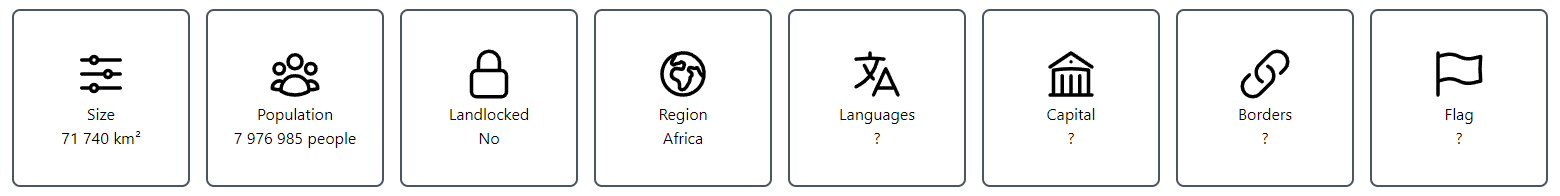
\includegraphics[width=.97\textwidth]{images/HintBoxes.jpg}
	\caption[HintBoxes]{HintBoxes - vlastní zpracování}
	\label{fig:sveltehintboxes}
\end{figure}

Komponenta \emph{CountryGuessInput.svelte} umožní uživateli zadání názvu země (uživatelova tipu). Začneme šablonou, kde vytvoříme formulářový prvek pro zadání tipu a~potvrzovací tlačítko. 
Dále také podmenu textového pole, které zobrazí nejpodobnější země na základě zadaného textu (filtrované země). Přidáme obslužné funkce pro akce a~události nad formulářem, které následně doimplementujeme.

\begin{figure}[htb]
	\centering
		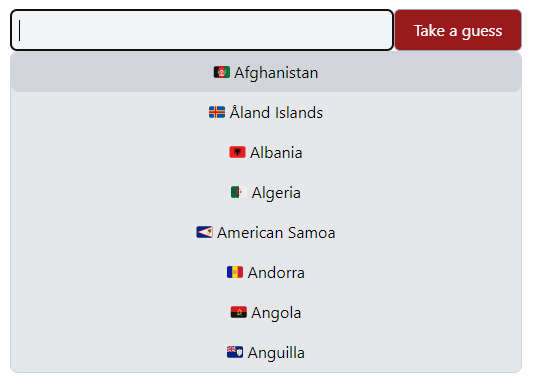
\includegraphics[width=.5\textwidth]{images/CountryGuessInput.jpg}
	\caption[CountryGuessInput]{CountryGuessInput - vlastní zpracování}
	\label{fig:sveltecountryguessinput}
\end{figure}

Ve skriptové části, na základě vstupu \emph{countries}, získáme pole všech zemí bez těch, které uživatel již hádal (\emph{countriesWithoutAlreadyGuessed}). 
Následně definujeme a~inicializujeme ostatní stavy komponenty. Po kliknutí na potvrzovací tlačítko zavoláme funkci \emph{handleGuessButtonClick}. 
V~tělě funkce zavoláme obslužnou funkci \emph{evaluateGuessAndUpdateState}, pomocí níž vyhodnotíme stav hry v~rodičovské komponentě. 
Dále také funkci \emph{handleChangeSelectedGuess}, která aktualizuje aktuální tip, filtrované země a~uzavře podmenu. 
Funkce \emph{handleInputChange} převede tip uživatele do daného formátu, aktualizuje aktuální tip a~filtrované země. Ovládání textového pole pomocí klávesnice umožní funkce \emph{handleKeyDown}.

V~pomocné funkci \emph{updateGuessAndFilteredCountries} nejprve získáme filtrované země podle uživatelova tipu. Pak aktualizujeme stavy \emph{currentGuess}, \emph{isValidGuess} a~\emph{filteredCountries}. 
Funkce \emph{clampSelectedGuessIndex} zajistí, aby index vybrané země byl v~požadovaném rozmezí (0 až počet filtrovaných zemí). 
K~modifikaci stavu \emph{selectedGuessIndex} použijeme funkci \emph{changeSelectedGuessIndex}, která index aktualizuje o~hodnotu předanou v~argumentu. 
Tip uživatele pomocí funkce \emph{convertToFormattedGuess} převedeme tak, aby začínal velkým písmenem a~zbytek řetezce byl složen z~malých písmen.

Pro zobrazení všech již hádaných zemí uživatelem vytvoříme komponentu GuessedCountriesList. 
Ze vstupních vlastností \emph{countries}, \emph{guessedCountries} a~\emph{randomCountry} získáme proměnnou \emph{enrichedGuessedCountries}. 
Jde o~uživatelem hádané země s~vlajkou a~vzdáleností od \emph{randomCountry}. K~převodu využijeme JS funkci z~jiného souboru. 
Vzdálenost zemí vypočteme pomocí knihovny \emph{calculate-distance-between-coordinates} \cite{distancebetweencoordinates}, která exportuje funkci \emph{getDistanceBetweenTwoPoints}. 
Proměnnou \emph{enrichedGuessedCountries} poté vykreslíme v~šabloně.

\begin{figure}[htb]
	\centering
		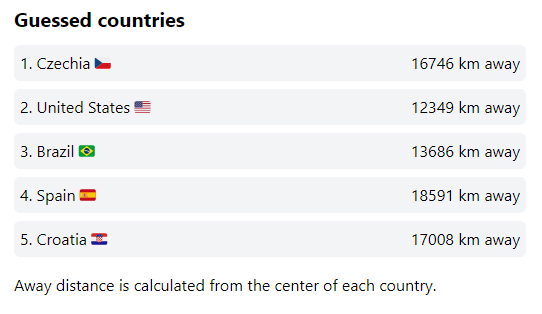
\includegraphics[width=.7\textwidth]{images/GuessedCountriesList.jpg}
	\caption[GuessedCountriesList]{GuessedCountriesList - vlastní zpracování}
	\label{fig:svelteguessedcountrieslist}
\end{figure}

Závěrem vytvoříme modální okna, která vykreslíme při výhře nebo prohře. Stavy \emph{isWinModalOpen} a~\emph{isLoseModalOpen} aktualizujeme uvnitř funkce \emph{handleEvaluateGuessAndUpdateState} v~CountryGuesser. 
Na základě těchto stavů podmíněně zobrazíme daná modální okna. Oběma oknům předáme \emph{randomCountry} a~obslužnou funkci \emph{handleClose}. Do výherního modálu také počet potřebných pokusů. 
V~jednotlivých komponentách (WinModal, LoseModal) vykreslíme komponentu BaseModal, která bude sloužit jako šablona pro obě okna. Do této komponenty pak předáme titulek, obsah modálu a~obslužnou metodu \emph{handleClose}. 
V~šabloně BaseModal vykreslíme základní strukturu modálního okna s~dynamickými vlastnostmi.

\subsubsection*{Routování a layout aplikace}

Aplikaci rozdělíme do tří částí: hlavičky, patičky a~samotného obsahu, v~němž vykreslíme jednotlivé komponenty. Uživatel se bude moci přepínat mezi jednotlivými stránkami přes navigační menu. 

Pro routování v~aplikaci využijeme knihovnu \emph{svelte-spa-router} \cite{sveltesparouterlib}. Nejprve vytvoříme seznam cest aplikace (\emph{appRoutes}).

\begin{prog}
// Část souboru appRoutes.ts

interface AppRoute \{
  name?: string;
  path: string;
  component: ComponentType;
\}

export const appRoutes: ReadonlyArray<AppRoute> = [
  \{
    name: 'Home',
    path: '/',
    component: Landing,
  \},
  \{
    name: 'Counter',
    path: '/counter',
    component: Counter,
  \},
  // Další cesty...
  \{
    path: '*',
    component: PageNotFound,
  \},
];
\end{prog}

Uvnitř hlavní komponenty transformujeme \emph{appRoutes} do požadovaného formátu (typu \emph{RouteDefinition}) a~výsledek uložíme do proměnné \emph{routes}. 
V~šabloně zobrazíme hlavičku, patičku a~\emph{Router}, kterému předáme proměnnou \emph{routes}. 
\emph{Router} následně vykreslí šablonu na základě aktuální URL adresy.

\begin{prog}
// Část souboru App.svelte

<script lang="ts">
  // Importy...

  // Vytvoření cest pro svelte-spa-router.
  const routes: RouteDefinition = appRoutes.reduce(
    (routesMap, route) => routesMap.set(route.path, wrap(\{
      component: route.component
    \})),
    new Map()
  );
</script>

<QueryClientProvider client=\{queryClient\}>
  <div class="min-h-screen flex flex-col">
    <Header />

    <main class="flex-grow p-8">
      <!-- Router vykresluje šablonu (komponentu) pro aktuální URL adresu. -->
      <Router \{routes\} />
    </main>

    <Footer />
  </div>
</QueryClientProvider>
\end{prog}

Hlavička zobrazí odkazy na jednotlivé stránky. Architekturu a~vzhled navigačního menu převezmeme např.~od Flowbite. 
V~rámci komponenty Header vypíšeme cesty aplikace pomocí HTML elementu a, na nějž přidáme atribut href. 
Dále přidáme také akce \emph{link} a~\emph{active}, které poskytuje \emph{svelte-spa-router}. 
Akci \emph{active} předáme objekt, kde přes vlastnosti \emph{className} a~\emph{inactiveClassName} nastavíme požadovanou CSS třídu podle toho, zda je odkaz aktivní nebo neaktivní. 
K~nastavení aria-current použijeme \emph{location} objekt ze \emph{svelte-spa-router}, díky kterému získáme aktuální URL.

\begin{prog}
// Část souboru Header.svelte

\{#each routes as route\}
  <li>
    <!-- svelte-spa-router poskytuje akce "link" a také "active". -->
    <!-- Akce active slouží k nastavení CSS na základě aktivního odkazu. -->
    <a
      href=\{route.path\}
      class="block py-2 pr-4 pl-3 lg:p-0"
      use:link
      use:active=\{\{
        className: 'STATICKÉ STYLY PRO AKTIVNÍ ODKAZ...',
        inactiveClassName: 'STATICKÉ STYLY PRO NEAKTIVNÍ ODKAZ...',
      \}\}
      aria-current=\{route.path === \$location ? 'page' : null\}
    >
      \{route.name\}
    </a>
  </li>
\{/each\}
\end{prog}

Stavy \emph{isMobileNavOpen} a~\emph{isDarkMode} umožní ovládat zobrazení mobilní navigace a~barevného režimu. K~uložení preference tmavého režimu využijeme LocalStorage v~prohlížeči. 
Logiku pro přepnutí barevného režimu zavoláme v~hooku \emph{beforeUpdate}. Tento hook se spustí po změně lokálního stavu, ale před aktualizací HTML.

\begin{prog}
// Část souboru Header.svelte

beforeUpdate(() => \{
  if (isDarkMode) \{
    document.documentElement.setAttribute('data-mode', 'dark');
    localStorage.setItem('data-mode', 'dark');
  \} else \{
    document.documentElement.removeAttribute('data-mode');
    localStorage.removeItem('data-mode');
  \}
\});
\end{prog}

\begin{zvyraznenyodstavec}
\subsection{Srovnání implementace aplikací}
% s čím se jak pracovalo, velikosti souborů, řádky, jak pomohla dokumentace

V této podkapitole se zaměříme na srovnání aspektů implementace aplikací v rámci vybraných frameworků. 
Cílem je provést detailnější srovnání s ohledem na poznatky z provedených implementací. 

Využití Angularu při implementaci aplikace se vyznačovalo objektově orientovaným přístupem, který umožňuje využít například výhodu zapouzdření. 
Nespornou výhodu tvořila modularita frameworku, která podporuje rozšiřitelnost a robustnost aplikace. 
Framework poskytuje nativní podporu pro router, formuláře, validace a mnoho dalších funcionalit, čímž snižuje závislost na třetích stranách. 
Angular, dle autora práce, oproti ostatním frameworkům nabízí intuitivnější syntax pro podmíněné vykreslení v šabloně. 
Framework také disponuje řadou metod životního cyklu, což může být výhodou. Na druhou stranu začátečník může být z množství metod životního cyklu zmatený. 
U stylování komponent Angular rozlišuje statické a dynamické styly, což umožňuje lepší organizaci a přehlednost. 
Při implementaci rozhodně nemůžeme opomenout Angular CLI, jenž zjednodušuje opakující se operace v rámci vývoje. 
Jako výhodu také můžeme uvést podporu jazyka TypeScript již v základu. 
Na druhou stranu Angular vyžaduje více konfigurace. Implementace je tak oproti dalším dvěma frameworkům nejdelší a nejsložitější. 
V rámci vývoje se ukázalo, že Angular je náročný na naučení a framework sám o sobě umožňuje programátorovi udělat mnoho chyb. 
Tomu rozhodně nepomáhá implementace reaktivity pomocí knihovny RxJS. 
Programátor rovněž musí počítat s tím, že Angular generuje element dané komponenty v DOM, což může zkomplikovat např. stylování. 
Angular neposkytuje možnost použití destrukturování při předávání vlastností. 
Tím pádem je třeba vždy předat všechny vlastnosti zvlášť nebo je uložit ve vhodnější datové struktuře (např. objektu).
Běhěm vývoje jsme také narazili na problém s neinicializováním vstupních vlastností, což může být problematické. 
Problém je řešitelný dvěma způsoby, z nichž ani jeden není zcela ideální.

% Angular:
% + OOP přístup (lze použít např. zapouzdření...)
% + nejintuitivnější práce s podmíněným vykreslením
% + výborná modularita, > robusnost aplikace
% + opravdu pestrý z hlediska funcionalit
% + podporuje nativně např. router, forms, validace, ...
% + hodně metod pro životní cyklus (nevýhodou je, že jich je opravdu dost...)
% + styly rozdělěny na static + dynamic
% + CLI
% + podporuje TypeScript jako default
% + předávání vlastností
% - velikost souborů (nejvíce řádků), moc konfigurace
% - těžší na naučení, hlavně složitější reaktivita s RxJS...
% - sám o sobě umožňuje programátorovi udělat mnoho chyb
% - vytváří element dané komponenty v DOM
% - nelze použít destructuring pro předávání vlastností
% - input je třeba vždy inicializovat (lze to obejít - bad practise)
% - během vývoje problém s vscode pluginem

Implementace v Reactu ukázala silné stránky v podobě silného ekosystému a velmi dobře propracovaných balíčků. 
React disponuje dokumentací na vysoké úrovni a internet je rovněž plný kvalitních návodů a tutoriálů. 
S tím souvisí i kvalitní chybové hlášky, které pomáhají programátorům řešit dané chyby. 
React poskytuje typy pro atributy běžných HTML elementů, což výrazně zjednodušuje a zefektivnǔje práci. 
Vlastnosti jsou v rámci vnořených komponent k dispozici ihned a jsou vždy aktualizované, což u dalších frameworků neplatí. 
Velkou výhodu představuje možnost použití destrukturování pro předávání vlastností. 
Jako výhodu lze také uvést modularitu, které dosáhneme při implmenetaci vlastních hooků. 
Nevýhody frameworku se projevily při vykreslování a využívání zabudovaných hooků. 
Při špatném použití vykreslovací techniky (pomocí \&\& nebo || operátorů) můžeme zobrazit nechtěné výsledky v DOM. 
V rámci funkce map nesmíme zapomenout každému elementu přidělit unikátní klíč. 
Co se týče hooků, především useEffect hook umožňuje programátorům snadné zavedení chyb, pokud není správně použit. 
S tím se rovněž pojí problémy se závislostmi useEffect a neintuitivní kontrola životního cyklu komponenty. 
Vývojáři také musí počítat s tím, že aktualizace stavů je vždy asynchronní. V praxi to znamená, že stav není aktualizován okamžitě. 
Jako nevýhodu můžeme uvést i předávání vlastností do rodičovské komponenty, které minimálně zpočátku může vypadat složitě.

% React:
% + nejvíce propracované knihovny a super ekosystém
% + kvalitní dokumentace, návody, tutoriály
% + nejlepší chybové hlášky
% + poskytuje typy pro atributy HTML elementů
% + props jsou k dostání ihned a jsou aktualizované
% + destructuring pro předávání vlastností
% + modularita pomocí hooků
% - sám o sobě umožňuje programátorovi udělat mnoho chyb (useEffect, key v map...)
% - špatné použití vykreslení (ternár, \&\&, ||) může způsobit problémy
% - useEffect a závislosti...
% - nejméně intuitivní kontrola lifecycle
% - aktualizace stavu je asynchronní
% - je třeba si zvyknout na předávání vlastností do rodiče

Implementace ve Svelte poukázala na jednoduchost a přímočarost tohoto frameworku. 
Syntax je velmi čitelná a bez zbytečného boilerplate kódu, což v porovnání s dalšími frameworky znamená nejkratší kód. 
Svelte elegantním způsobem řeší předávání vlastností mezi komponentami. 
Díky \$\$restProps můžeme získat všechny vlastnosti, které nejsou explicitně deklarovány. 
Musíme si však dávat pozor na to, že při předání nekorektní vlastnosti do komponenty můžeme narazit na problémy. 
Reactive statement dokáže reagovat na změny hodnot v rámci svého těla, což je velice efektivní a užitečné. 
Svelte také oproti předchozím frameworkům nabízí přehledný systém metod životního cyklu a modifikaci DOM přes akce. 
V neposlední řadě je třeba zmínit jednoduchý each blok a observables systém, který vývojářům zbytečně nekomplikuje práci.
Mezi slabší stránky frameworku rozhodně patří jeho ekosystém a komunita, která je nejmenší a zatím se rozvíjí. 
Svelte proto disponuje nejméně kvalitními knihovnami určené tomuto frameworku. 
Syntax může být někdy matoucí, například klíčové slovo export u vstupních vlastností, nebo zvláštní syntax \#if, :else if, :else, /if. 
Vývojáři musí mít na paměti modifikaci vstupních vlastností po jejich aktualizaci, kterou je třeba provést reaktivně. 
V neposlední řadě můžeme zmínit nevýhody při práci s TypeScriptem. Pro importování TS typů používáme ve Svelte navíc klíčové slovo type. 
Do TS souboru nelze importovat TS typ ze Svelte komponenty, takový typ pak zakládáme v rámci context="'module"' skriptu v komponentě.
Při porovnání s ostatními frameworky, Svelte disponuje hůře otypovanými událostmi, což prodlužuje práci v obslužných funkcích.

% Svelte:
% + nejméně boilerplate kódu -> opravdu jednoduchý na naučení (obvykle nejkratší kód)
% + easy to read syntax
% + nejjednodušší předávání vlastností (nahoru i dolů)
% + restProps -> výhoda i nevýhoda (při předání nekorektní vlastnosti)
% + reactive statement funguje dle jeho implemenetace
% + vyváženost u lifecycle metod (fungují jak mají a jsou jednoduché)
% + modifikace/poslouchání DOM přes akce
% + intuituvní for (each) - jednoduchý, ale mocný
% + jednoduchý systém observables
% - nejmladší s nejmenší komunitou, nejčastěji potkáme chyby (které nemusí být hned vyřešeny)
% - nejslabší knihovny (router není tak vyšperkovaný, balíčkům chybí funkce...)
% - syntax je někdy matoucí (export u input vlastností, if, else if, else, /if divná syntaxe)
% - modifikace inputů musí být prováděna pomocí reactive statementu
% - znaky navíc při importu TS typů (type)
% - do ts souboru nelze importovat TS typ ze Svelte komponenty (typ musí být založen v context="module" skriptu)
% - nejméně otypované handlery eventů

Srovnání implementace aplikací v rámci vybraných frameworků ukázalo, že každý framework má své přednosti i nedostatky. 
Angular se vyznačuje robustností a modularitou, což může být výhodou zejména u větších projektů. 
React disponuje obrovským ekosystémem i kvalitními knihovnami, a to mohou ocenit především začátečníci. 
Svelte zase nabízí jednoduchost, přímočarost a může být vhodný spíše pro menší projekty.
\end{zvyraznenyodstavec}